% concatenated from FPPsublinear.tex
%%%%% section{Preamble}
\documentclass[12 pt]{amsart}
% --c \documentclass[11pt,letterpaper,oneside]{amsart}
  \usepackage[utf8]{inputenc}
  \usepackage[margin=3cm]{geometry}
  \setlength{\textheight}{21cm}
  \setlength{\textwidth}{15cm}  
  
%\usepackage{titletoc, tocloft}
%\setlength{\cftsubsecindent}{1cm}
%\setlength{\cftsubsubsecindent}{2cm}
%\dottedcontents{section}[1.5em]{}{1.3em}{.6em}


\setcounter{tocdepth}{1}
\makeatletter
\def\l@subsection{\@tocline{1}{0pt}{2pc}{1pc}{}}
\def\l@subsubsection{\@tocline{2}{0pt}{2pc}{1pc}{}}
\makeatother

  %subsection{Packages}
  \usepackage{stmaryrd}
\usepackage{amsmath,amssymb,amsthm, mathrsfs, mathtools, bbold, mathbbol}
\usepackage{amscd,mathtools}
\usepackage{comment}
  \usepackage{geometry}
  \usepackage{graphicx,epstopdf}
  \usepackage{color,xcolor}
  \usepackage{enumerate}
  \usepackage{xspace}
  \usepackage{tipa}
  \usepackage[user,titleref]{zref}
%  \usepackage{showlabels}
 \usepackage{soul}
 \usepackage{xcolor}
  %\usepackage{amscd}
 % \usepackage[notcite,notref]{showkeys}
  \usepackage{epsfig}
 % \usepackage{pinlabel}
 % \usepackage[all]{xy}
  
\usepackage{tikz}
\usetikzlibrary{shapes.geometric}
\usetikzlibrary{angles}


\usepackage{caption, subcaption}
\usepackage{tikz-cd}
\usetikzlibrary{calc,decorations.pathreplacing}
\usepackage{tikz}
\usetikzlibrary{calc}
\usetikzlibrary{arrows}
\usetikzlibrary{decorations.pathreplacing}
\usetikzlibrary{intersections}


%\usepackage[dvips]{graphicx}
%\usepackage{color}              % Need the color package
%\usepackage{epsfig}
%
%\usepackage{tikz}
%\usetikzlibrary{calc,through,backgrounds, arrows}
%\usetikzlibrary{decorations.pathmorphing, decorations.pathreplacing,positioning,fit}. 
%

\usepackage{mathrsfs}
\usetikzlibrary{matrix}
\usetikzlibrary{positioning}
\DeclareMathAlphabet{\pazocal}{OMS}{zplm}{m}{n}
% set arrows as stealth fighter jets
\tikzset{>=stealth}
  %\usepackage{color}
  %\definecolor{darkgreen}{rgb}{0, 0.40, 0}

  %\usepackage{amsthm} %%% Defines \theoremstyle
  %\usepackage{amsmath} %%% Defines \numberwithin, \operatorname
  %\usepackage{amssymb} %%% Defines \mathbb

  %\usepackage{psfrag}

  \usepackage{hyperref}

  \hypersetup{
    colorlinks=true,
    linkcolor=blue,
    filecolor=magenta,      
    urlcolor=cyan,
    citecolor=purple,
    pdftitle={Overleaf Example},
    pdfpagemode=FullScreen,
    }

\usepackage{float}


  %%%%% subsection{Fonts} 

  %% Calligraphy 

  \newcommand{\calA}{\mathcal{A}}
  \newcommand{\calB}{\mathcal{B}}
  \newcommand{\calC}{\mathcal{C}}
  \newcommand{\calD}{\mathcal{D}}
  \newcommand{\calE}{\mathcal{E}}
  \newcommand{\calF}{\mathcal{F}}
  \newcommand{\calG}{\mathcal{G}}
  \newcommand{\calH}{\mathcal{H}}
  \newcommand{\calI}{\mathcal{I}}
  \newcommand{\calJ}{\mathcal{J}}
  \newcommand{\calK}{\mathcal{K}}
  \newcommand{\calL}{\mathcal{L}}
  \newcommand{\calM}{\mathcal{M}}
  \newcommand{\calN}{\mathcal{N}}
  \newcommand{\calO}{\mathcal{O}}
  \newcommand{\calP}{\mathcal{P}}
  \newcommand{\calQ}{\mathcal{Q}}
  \newcommand{\calR}{\mathcal{R}}
  \newcommand{\calS}{\mathcal{S}}
  \newcommand{\calT}{\mathcal{T}}
  \newcommand{\calU}{\mathcal{U}}
    \newcommand{\calV}{\mathcal{V}}
  \newcommand{\calW}{\mathcal{W}}
  \newcommand{\calX}{\mathcal{X}}
  \newcommand{\calY}{\mathcal{Y}}
  \newcommand{\calZ}{\mathcal{Z}}
  
  %%%%this paper
  

  

    \newcommand{\Uout}{ \calU_{\rm \, Out}}
    \newcommand{\pin}{\partial_{\rm \, In} }
    \newcommand{\pout}{\partial_{\rm Out}} 
  \newcommand{\Rin}{R^{\rm in}}

  %% Math Bold

  \renewcommand{\AA}{\mathbb{A}}
  \newcommand{\BB}{\mathbb{B}}
  \newcommand{\CC}{\mathbb{C}}
  \newcommand{\DD}{\mathbb{D}}
  \newcommand{\EE}{\mathbb{E}}
  \newcommand{\FF}{\mathbb{F}}
  \newcommand{\HH}{\mathbb{H}}
  \newcommand{\KK}{\mathbb{K}}
  \newcommand{\MM}{\mathbb{M}}
  \newcommand{\NN}{\mathbb{N}}
  \newcommand{\OO}{\mathbb{O}} 
  \newcommand{\PP}{\mathbb{P}}
  \newcommand{\QQ}{\mathbb{Q}}
  \newcommand{\RR}{\mathbb{R}}
  \renewcommand{\SS}{\mathbb{S}}
  \newcommand{\TT}{\mathbb{T}}
  \newcommand{\VV}{\mathbb{V}}
  \newcommand{\WW}{\mathbb{W}}
  \newcommand{\XX}{\mathbb{X}}
  \newcommand{\YY}{\mathbb{Y}}
  \newcommand{\ZZ}{\mathbb{Z}}

  %% Text bold
  
  \newcommand{\bfa}{\textbf{a}}
  \newcommand{\bfb}{\textbf{b}}
  \newcommand{\bfc}{\textbf{c}}  
  \newcommand{\bfd}{\textbf{d}} 
  \newcommand{\bfx}{\textbf{x}}  
  \newcommand{\bfz}{\textbf{z}}  

  %% Gothic letters
  
  \newcommand{\gothic}{\mathfrak}
  \newcommand{\Ga}{{\gothic a}}
  \newcommand{\Gb}{{\gothic b}}
  \newcommand{\Gc}{{\gothic c}}
  \newcommand{\Gd}{{\gothic d}}
  \newcommand{\Ge}{{\gothic e}}
  \newcommand{\Gf}{{\gothic f}}
  \newcommand{\GF}{{\gothic F}}
  \newcommand{\Gg}{{\gothic g}}
  \newcommand{\Gh}{{\gothic h}}
  \newcommand{\Gi}{{\gothic i}}
  \newcommand{\Gj}{{\gothic j}}
  \newcommand{\Gk}{{\gothic k}}
  \newcommand{\Gl}{{\gothic l}}
  \newcommand{\Gm}{{\gothic m}}
  \newcommand{\gn}{{\gothic n}}
  \newcommand{\go}{{\gothic o}}
  \newcommand{\Gp}{{\gothic p}}
  \newcommand{\Gq}{{\gothic q}}
  \newcommand{\Gr}{{\gothic r}}
  \newcommand{\Gs}{{\gothic s}}
  \newcommand{\Gt}{{\gothic t}}
  \newcommand{\Gu}{{\gothic u}}
  \newcommand{\gv}{{\gothic v}}
  \newcommand{\Gw}{{\gothic w}}
  \newcommand{\gx}{{\gothic x}}
  \newcommand{\gy}{{\gothic y}}
  \newcommand{\Gz}{{\gothic z}}
  \newcommand{\GS}{{\gothic S}}
  

\newcommand{\rE} {{\mathcal{E} }}
\newcommand{\rEB} {{\mathcal{EB} }}

  %%%%%% subsection{Standard Math}

  %% Environments and Numbering 

  \newtheorem{theorem}{Theorem}[section]
  \newtheorem{proposition}[theorem]{Proposition}
  \newtheorem{corollary}[theorem]{Corollary}
  \newtheorem{lemma}[theorem]{Lemma}
  \newtheorem{conjecture}[theorem]{Conjecture}
  \newtheorem{problem}[theorem]{Problem}
  \newtheorem{question}[theorem]{Question}
  \newtheorem{claim}[theorem]{Claim}
  \newtheorem{subclaim}[theorem]{Subclaim}
  \newtheorem*{claim*}{Claim}

  \newtheorem{introthm}{Theorem}
  \newtheorem{introcor}[introthm]{Corollary}
  \newtheorem{introprop}[introthm]{Proposition} 
  \newtheorem{introques}[introthm]{Question} 
  \renewcommand{\theintrothm}{\Alph{introthm}}
  \renewcommand{\theintrocor}{\Alph{introcor}}
  \renewcommand{\theintroprop}{\Alph{introprop}}
  \renewcommand{\theintroques}{\Alph{introques}}

  \theoremstyle{definition}
  \newtheorem{definition}[theorem]{Definition}
  \newtheorem{exercise}[theorem]{Exercise}
  \newtheorem{example}[theorem]{Example}
  \newtheorem{fact}[theorem]{Fact}
  \newtheorem*{question*}{Question}
  \newtheorem*{answer*}{Answer}
  \newtheorem*{application*}{Application}
  \newtheorem{notation}[theorem]{Notation}

  \theoremstyle{remark}
  \newtheorem{remark}[theorem]{Remark}
  \newtheorem*{remark*}{Remark}
  
%  \numberwithin{equation}{section}

  %% References

  \newcommand{\secref}[1]{Section~\ref{#1}}
  \newcommand{\thmref}[1]{Theorem~\ref{#1}}
  \newcommand{\corref}[1]{Corollary~\ref{#1}}
  \newcommand{\lemref}[1]{Lemma~\ref{#1}}
  \newcommand{\propref}[1]{Proposition~\ref{#1}}
  \newcommand{\clmref}[1]{Claim~\ref{#1}}
  \newcommand{\remref}[1]{Remark~\ref{#1}}
  \newcommand{\exaref}[1]{Example~\ref{#1}}
  \newcommand{\facref}[1]{Fact~\ref{#1}}
  \newcommand{\exref}[1]{Exercise~\ref{#1}}
  \newcommand{\figref}[1]{Figure~\ref{#1}}
  \newcommand{\defref}[1]{Definition~\ref{#1}}
  \newcommand{\probref}[1]{Problem~\ref{#1}}
  \newcommand{\eqnref}[1]{Equation~\eqref{#1}}
  \newcommand{\mf}[1]{\mathfrak{#1}}
  \newcommand{\fo}{{\mathfrak{o}}}
  \newcommand{\opi}{{\overline \pi}}
    \newcommand{\oX}{{\overline X}}

  %% Operators:

  \DeclareMathOperator{\Mod}{Mod}
    \DeclareMathOperator{\Sat}{Sat}
  \DeclareMathOperator{\Ext}{Ext}
  \DeclareMathOperator{\Hyp}{Hyp}
  \DeclareMathOperator{\special subset}{special subset}
  \DeclareMathOperator{\area}{area}
  \DeclareMathOperator{\I}{i}
  \DeclareMathOperator{\Vol}{Vol}
  \DeclareMathOperator{\Area}{Area}
  \DeclareMathOperator{\twist}{twist}
  \DeclareMathOperator{\tw}{tw}
  \DeclareMathOperator{\fold}{fold}
  \DeclareMathOperator{\green}{stretch}

  %% Inequalities:

  \newcommand{\emul}{\stackrel{{}_\ast}{\asymp}}
  \newcommand{\gmul}{\stackrel{{}_\ast}{\succ}}
  \newcommand{\lmul}{\stackrel{{}_\ast}{\prec}}
  \newcommand{\eadd}{\stackrel{{}_+}{\asymp}}
  \newcommand{\gadd}{\stackrel{{}_+}{\succ}}
  \newcommand{\ladd}{\stackrel{{}_+}{\prec}}

  %% Relations

  \newcommand{\isotopic}{\mathrel{\approx}}
  \newcommand{\homeo}{\mathrel{\cong}} % Homeomorphism
  \newcommand{\nhomeo}{\mathrel{\not\cong}}
  \newcommand{\isom}{\cong} % Isomorphism
  \newcommand{\disjoint}{\mathbin{\amalg}} % Disjointness
  \newcommand{\cross}{\times}
  \newcommand{\cutby}{\mathbin{\rule[.023 in]{.12 in}{.02 in}}} 
  \newcommand{\derivative}[2]{ \frac{{\partial{#1}}{\partial{#2}} } }
  \newcommand{\pka}{\partial_{\kappa}}

  %% Spaces

  \newcommand{\Aut}{\ensuremath{\operatorname{Aut}}\xspace} 
       % Automorphism group
 % \newcommand{\Out}{\ensuremath{\operatorname{Out}}\xspace} 
       % Outer automorphism group
  \newcommand{\Inn}{\ensuremath{\operatorname{Inn}}\xspace} 
      % Inner automorphism group

   \newcommand{\GL}{\ensuremath{\operatorname{GL}}\xspace} 
       % General linear
  \newcommand{\SL}{\ensuremath{\operatorname{SL}}\xspace} 
       % Special linear
  \newcommand{\PGL}{\ensuremath{\operatorname{PGL}}\xspace} 
         % Projective general linear
  \newcommand{\PSL}{\ensuremath{\operatorname{PSL}}\xspace} 
       % Projective special linear
  \newcommand{\SO}{\ensuremath{\operatorname{SO}}\xspace} 
       % Special orthogonal

  \newcommand{\Map}{\ensuremath{\operatorname{Map}}\xspace}  
  \newcommand{\MCG}{\ensuremath{\mathcal{MCG}}\xspace}  
       % Mapping class group
  \newcommand{\AC}{\ensuremath{\mathcal{AC}}\xspace} 
       % Arc and Curve Complex

  \newcommand{\T}{\ensuremath{\mathcal{T}}\xspace} 
       % Teichmuller space
  \newcommand{\MF}{\ensuremath{\mathcal{MF}}\xspace} 
       % Measured foliations
  \newcommand{\PMF}{\ensuremath{\mathcal{PMF}}\xspace} 
       % Projectively measured foliations
  \newcommand{\ML}{\ensuremath{\mathcal{ML}}\xspace} 
         % Ditto for laminations
  \newcommand{\FL}{\ensuremath{\mathcal{FL}}\xspace} 
       % Filling laminations
  \newcommand{\EL}{\ensuremath{\mathcal{EL}}\xspace} 
        % Ending laminations
  \newcommand{\PML}{\ensuremath{\mathcal{PML}}\xspace}  
        % Projectivised measured laminations

  \newcommand{\Mark}{\ensuremath{\mathcal{MK}}\xspace}  
        % Marking graph

%% Long Words  

  \newcommand{\Teich}{{Teichm\"uller }} % A Nazi dude
  \hyphenation{geo-desics} 
  \newcommand{\Ham}{{Hamenst\"adt }}


  %% Constants

  \newcommand{\sA}{{\sf A}}   
  \newcommand{\sB}{{\sf B}}   
  \newcommand{\sC}{{\sf C}}   
  \newcommand{\sD}{{\sf D}}     
  \newcommand{\sE}{{\sf E}}   
  \newcommand{\sF}{{\sf F}}   
  \newcommand{\sG}{{\sf G}}   
  \newcommand{\sH}{{\sf H}}     
  \newcommand{\sI}{{\sf I}}   
  \newcommand{\sJ}{{\sf J}}   
 \newcommand{\sK}{{\sf K}}   
  \newcommand{\sL}{{\sf L}}     
  \newcommand{\sM}{{\sf M}}   
  \newcommand{\sN}{{\sf N}}   
  \newcommand{\sO}{{\sf O}}   
  \newcommand{\sP}{{\sf P}}       
  \newcommand{\sQ}{{\sf Q}}   
  \newcommand{\sR}{{\sf R}}   
  \newcommand{\sS}{{\sf S}}     
  \newcommand{\sT}{{\sf T}}   
  \newcommand{\sU}{{\sf U}}   
  \newcommand{\sV}{{\sf V}}   
  \newcommand{\sW}{{\sf W}}     
  \newcommand{\sX}{{\sf X}}   
  \newcommand{\sY}{{\sf Y}}   
  \newcommand{\sZ}{{\sf Z}}     
  
  
  \renewcommand{\bfa}{{\sf a}}   
   \renewcommand{\bfd}{{\sf d}}  

  \newcommand{\bb}{{\sf b}}   
  \newcommand{\cc}{{\sf c}}   
  \newcommand{\dd}{{\sf d}}     
  \newcommand{\ee}{{\sf e}}   
  \newcommand{\ff}{{\sf f}}   
  %\renewcommand{\gg}{{\sf g}}   
  \newcommand{\hh}{{\sf h}}     
  \newcommand{\ii}{{\sf Ii}}   
  \newcommand{\jj}{{\sf j}}   
  \newcommand{\kk}{{\sf k}}   
  \renewcommand{\ll}{{\sf l}}     
  \newcommand{\mm}{{\sf m}}   
  \newcommand{\nn}{{\sf n}}   
  \newcommand{\oo}{{\sf o}}   
  \newcommand{\pp}{{\sf p}}       
  \newcommand{\qq}{{\sf q}}   
  \newcommand{\rr}{{\sf r}}   
  \renewcommand{\ss}{{\sf s}}     
  \renewcommand{\tt}{{\sf t}}   
  \newcommand{\uu}{{\sf u}}   
  \newcommand{\vv}{{\sf v}}   
  \newcommand{\ww}{{\sf w}}     
  \newcommand{\xx}{{\sf x}}   
  \newcommand{\yy}{{\sf y}}   
  \newcommand{\zz}{{\sf z}}   
      
  \newcommand{\radius}{{\sf r}}


%% Distances 

  \newcommand{\dL}{{d_L}} 
  \newcommand{\dT}{{d_T}} 
  \newcommand{\dS}{{d_S}} 


  %% Bars

  \newcommand{\balpha}{{\overline \alpha}}
  \newcommand{\bbeta}{{\overline \beta}}
  \newcommand{\bgamma}{{\overline \gamma}}
  \newcommand{\bphi}{{\overline \phi}}  
  \newcommand{\bnu}{{\overline \nu}}    
  \newcommand{\ba}{{\overline a}}
  \newcommand{\bc}{{\overline c}}
  \newcommand{\bd}{{\overline d}}  
  \newcommand{\be}{{\overline e}}
  \renewcommand{\bf}{{\overline f}}
  \newcommand{\bk}{{\overline k}}  
  \newcommand{\bp}{{\overline p}}
  \newcommand{\bq}{{\overline q}}
  \newcommand{\bx}{{\overline x}}
   \newcommand{\by}{{\overline y}}
   \newcommand{\bz}{{\overline z}}
   \newcommand{\bw}{{\overline w}}
   \newcommand{\bG}{{\overline \calG}}          
   \newcommand{\bI}{{\overline I}}  
   \newcommand{\oG}{{\overline \Gamma}}
   \newcommand{\eventual}{{\stackrel{e}{=}}}


  \newcommand{\ua}{{\underline a}}
  \newcommand{\ub}{{\underline b}}
  \newcommand{\uc}{{\underline c}}
    \newcommand{\oC}{{\overline C}}
  \newcommand{\supp}{{\rm supp}}
  \newcommand{\pf}{{\partial_{\rm f}}}
    \newcommand{\ps}{{\pc}}
  \newcommand{\pQ}{{\partial_{\rm f} Q}}

  %% Others:
\DeclareMathOperator{\Core}{Core}
\DeclareMathOperator{\Outer}{CV}
\DeclareMathOperator{\out}{Out}
\DeclareMathOperator{\diam}{diam}
\DeclareMathOperator{\Cay}{Cay}
\DeclareMathOperator{\Pen}{Pen}
\DeclareMathOperator{\C}{C}
\DeclareMathOperator{\deep}{deep}
\DeclareMathOperator{\trans}{trans}



\newcommand{\CV}{{\Outer_{\! n}}}
\newcommand{\Out}{\out(\F)}
  %------
  % Don't mess with this unless you know what you're doing.
  % (It creates a squarish vertically centered dot that can be used to
  %  indicate a free parameter.)
    
  \newcommand{\param}{{\mathchoice{\mkern1mu\mbox{\raise2.2pt\hbox{$
  \centerdot$}}
  \mkern1mu}{\mkern1mu\mbox{\raise2.2pt\hbox{$\centerdot$}}\mkern1mu}{
  \mkern1.5mu\centerdot\mkern1.5mu}{\mkern1.5mu\centerdot\mkern1.5mu}}}
  %------

\DeclarePairedDelimiterX{\norm}[1]{\lvert}{\rvert}{#1}
\DeclarePairedDelimiterX{\Norm}[1]{\lVert}{\rVert}{#1}

  \renewcommand{\setminus}{{\smallsetminus}}
  \renewcommand{\th}{{\rm th}}
%  \newcommand{\st}{\mathbin{\mid}} 
  \newcommand{\ST}{\mathbin{\Big|}} 
  \newcommand{\from}{\colon\thinspace} 
  \newcommand{\ep}{\epsilon}
  \newcommand{\bdy}{\partial} 
  \newcommand{\vis}{\bdy_\infty}
  \newcommand{\F}{{\FF_n}} 
  \newcommand{\ra}{{\rightarrow}}
  %\newcommand{\A}{{A(\Gamma)}}
  \newcommand{\ga}{{\gamma}}
  \newcommand{\bdf}{{\partial_{f} }}
 \newcommand{\pc}{{ \partial_{c} }}
 \newcommand{\hG}{{\hat{G}}}
  \newcommand{\hu}{{\hat{u}}}
    \newcommand{\hv}{{\hat{v}}}
      \newcommand{\hw}{{\hat{w}}}
 
 \newcommand\tab[1][1cm]{\hspace*{#1}}
\newcommand{\cat}[1]{{\mathscr{#1}}}
\newcommand{\D}{\delta}
\newcommand{\R}{\mathbb{R}}
\newcommand{\A}{\alpha}
\newcommand{\B}{\beta}
\newcommand{\p}{\partial}
\newcommand{\K}{\kappa}
\newcommand{\n}{\eta}
\newcommand{\hd}{\hat{d}}
\newcommand{\hX}{\widehat{X}}

\newcommand{\ob}{\mathfrak{o}}

%\newcommand{\CAT}{\ensuremath{\operatorname{CAT}(0)}\xspace}         
    
%  \newcommand{\CV}{{\Outer_{\! }}}
%  \DeclareMathOperator{\out}{Out}
%   \newcommand{\Out}{\out(\F)}  

\newcommand{\myGlobalTransformation}[2]
{
    \pgftransformcm{1}{0}{0.5}{0.3}{\pgfpoint{#1}{#2}}
}

    
%  \newcommand{\param}{{\mathchoice{\mkern1mu\mbox{\raise2.2pt\hbox{$
%  \centerdot$}}
%  \mkern1mu}{\mkern1mu\mbox{\raise2.2pt\hbox{$\centerdot$}}\mkern1mu}{
%  \mkern1.5mu\centerdot\mkern1.5mu}{\mkern1.5mu\centerdot\mkern1.5mu}}}
%  %------


 
\newcommand{\CAT}{\ensuremath{\operatorname{CAT}(0)}\xspace}         
    
%\newcommand{\ps}{\partial_{s}}
  
\newcommand{\Ccom}[1]{\Cmod\marginpar{\color{red}\tiny #1 --gt}} 
\newcommand{\Cmod}{$\textcolor{red}{\clubsuit}$} 

\newcommand{\Kcom}[1]{\Kmod\marginpar{\color{black}\tiny #1 --kr}} 
\newcommand{\Kmod}{$\textcolor{black}{\clubsuit}$} 

\newcommand{\Ycom}[1]{\Ymod\marginpar{\color{blue}\tiny #1 --yq}} 
\newcommand{\Ymod}{$\textcolor{blue}{\clubsuit}$} 

%%%%%%%%%%%%%%%%%%%preamble added by Yulan ends here
\title[Sublinearly Morse geodesics and First Passage Percolation]{Sublinear Morse geodesics and First Passage Percolation}
\author{Sagnik Jana}
 \address{Department of Mathematics,  University of Tennessee at Knoxville, Knoxville, TN, USA}
\email{sjana1@vols.utk.edu}

 
  \author{Yulan Qing}
 %\thanks{grants}
 \address{Department of Mathematics,  University of Tennessee at Knoxville, Knoxville, TN, USA}
 \email{yqing@utk.edu}
 


\begin{document}
\maketitle
\begin{abstract}
Given an infinite connected graph, a way to randomly perturb its metric is to assign random i.i.d. lengths to the edges of the graph. Assume that the graph is infinite and of bounded degree. Assume also strict positivity and finite expectation of the edge length distribution and existence of a sublinearly Morse bi-infinite geodesic line, we prove that  almost surely there exists a bi-infinite geodesic line. This generalizes a previous result of \cite{BT17} regarding Morse geodesics.  
\end{abstract}

\section{Introduction}
First passage percolation is a model of random perturbation of a given metric graph. In this paper, we shall restrict to the simplest model, where random i.i.d lengths are assigned to the edges of a fixed graph,  and analyse the existence of infinite geodesic lines. We refer to \cite{ADH15},\cite{GK12},\cite{Kesten} for background and references.

We recall here how first passage percolation is defined following \cite{BT17}. We consider a connected non-oriented graph $X$, whose set of vertices and edges are denoted by $V$ and $E$, respectively. For every function $\omega: E \rightarrow(0, \infty)$, we equip $V$ with the weighted graph metric $d_{\omega}$, where each edge $e$ has weight $\omega(e)$. In other words, for every $v_{1}, v_{2} \in V, d_{\omega}\left(v_{1}, v_{2}\right)$ is defined as the infimum over all path $\gamma=\left(e_{1}, \ldots, e_{m}\right)$ joining $v_{1}$ to $v_{2}$ of $|\gamma|_{\omega}:=\sum_{i=1}^{m} \omega\left(e_{i}\right)$. We note that the infimum is always realized as a consequence of the bounded degree assumption. The graph metric on $X$ corresponds to the case where $\omega =1$, in this case, we denote the metric as $d$. Our model consists in choosing independently at random the weights $\omega(e)$ according to the probability measure defined on the set of all weight functions $\omega$. We refer to section ~\ref{sec23} for formal details.  %We let $\nu$ be a probability measure supported on $[0, \infty)$. Our model consists in choosing independently at random the weights $\omega(e)$ according to $\nu$. More formally, we equip the space $\Omega=[0, \infty)^{E}$ with the product probability that we denote by $\mathbb{P}$.

%A famous open problem in percolation theory is whether with positive probability, first passage percolation on $\mathbb{Z}^{2}$ admits a bi-infinite geodesic. In his Saint-Flour course, Kesten attributes this question to Furstenberg. Licea and Newman \cite{LN96} made partial progress on this problem, which is still open, and mentioned that the conjecture that there are no such geodesics arose independently in the physics community studying spin glass. \cite{WW} proved absence of two sided infinite geodesic in a half plane, assuming the lengths distribution is continuously distributed with a finite mean.

%For Riemannian manifolds, the existence of bi-infinite geodesics is influenced by the curvature of the space. It is well-known that complete simply connected non-positively curved Riemannian manifolds (such as the Euclidean space $\mathbb{R}^{n}$ or the hyperbolic space $\mathbb{H}^{n}$) admit bi-infinite geodesics. Therefore, simply connected manifolds without two-sided geodesics must have positively curved regions. It is easy to come up with examples of complete Riemannian surfaces with bubble-like structures that create short cuts avoiding larger and larger balls around some origin. See \cite{Ballman} for background.

Let $X$ be a simplicial graph. Recall that a path $\gamma=\left(e_{1}, \ldots, e_{n}\right)$ between two vertices $x, y$ is a sequence of consecutive edges joining $x$ to $y$. We write
\[x=\gamma(0), \ldots, \gamma(n)=y\]
to mean the set of vertices such that for all $0 \leq i<n, \gamma(i)$ and $\gamma(i+1)$ are joined by the edge $e_{i+1}$. For all $i<j$, we shall also denote by $\gamma([i, j])$ the sub path $\left(e_{i+1}, \ldots, e_{j}\right)$ joining $\gamma(i)$ to $\gamma(j)$. Let $X_\omega$ denotes the graph $X$ with edge lengths $\omega(e)$ for each edge $e$.\newline
A bi-infinite geodesic is a geodesic which is doubly infinite that is, its vertices are indexed by $\mathbb{Z}$. It was conjectured that under i.i.d lengths of edges, almost surely there are no bi-infinite geodesics in FPP on $\mathbb{Z}^2.$ See \cite{Kesten} for more details. For negatively curved spaces, the situation changes dramatically. In \cite{WW}, Wehr proved that almost surely there is no bi-infinite geodesic which lies entirely in the upper half Euclidean plane. 

On the other hand, \cite{BT17} established the existence of bi-infinite geodesic line in the affirmative if we assume the existence of a Morse quasi-geodesic line before the percolation. In this case the geometric property of a Morse quasi-geodesic line strongly informs how it behaves after the percolation. We are thus inspired by the proof and show in this paper that even weaker assumptions suffices. That is, we suppose instead there is a geodesic line whose Morse probably weakens as it extends to infinity. This class of quasi-geodesics were constructed recently by \cite{QRT1,QRT2} and named \emph{sublinearly Morse } quasi-geodesics. The construction roughly replaces bounded neighborhood with a sublinear neighborhood with respect to the distance to the origin. In this paper, we prove
\begin{introthm}\label{introthm1}
Let $X$ be an infinite connected graph with bounded degree. Assume $\EE \omega_e < \infty$ and $\nu(0) = 0$. If $X$ contains a sublinearly Morse bi-infinite quasi-geodesic line, then for almost every $\omega$, there is a bi-infinite geodesic ray in $X_\omega$.
\end{introthm}
The proof is analogous to that of \cite{BT17}. We first offer a new property of sublinearly Morse geodesic rays and lines, which we refer to as middle recurrence. The name comes from the analogous property used in \cite{BT17}. The property is first exhibited by \cite{DMS} with an improved proof by \cite{ADT}. Using the middle recurrence, we derive a pointed superlinear divergence property when then is used in the main proof. In an upcoming paper, we aim to study whether sublinearly Morse directions are preserved under first passage percolation.
\subsection*{History}
For the Cayley graph of $\ZZ^2$ with respect to standard generators, first passage percolation was introduced by Hammersley and Welsh \cite{HW65}.  Benjamini, Tessera, and Zeitouni \cite{BZ12, BT17} studied the question in Gromov hyperbolic spaces and a number of questions have been raised there. In particular, \cite{BZ12} established the tightness of fluctuations of the passage time from the center to the boundary of a large ball, and \cite{BT17} established the almost sure existence of bi-geodesics in hyperbolic spaces. Recently Basu-Mj \cite{BM22} studied the first passage percolation on Gromov hyperbolic group $G$ with boundary equipped with the Patterson-Sullivan measure $\nu$. They showed that the variance of the first passage time grows linearly with word distance along word geodesic rays in every fixed boundary direction.

The sublinearly Morse boundary is a  geometric boundary construction that generalize the Gromov boundary. It is shown to be always quasi-isometrically invariant and  metrizable, and is frequently a group-invariant topological model for suitable random walks on the associated group. In comparison, Morse boundary, constructed in \cite{Morse, contracting}, in comparison, often lacks metrizability and Poisson boundary realization property.   Meanwhile, the genericity of a more geometric flavor is also exhibited for sublinearly Morse boundaries. In \cite{GQR22}, genericity of sublinearly Morse directions under Patterson Sullivan measure was shown to hold in the more general context of actions which admit a strongly contracting element. In fact, the results in \cite{GQR22} concerning stationary measures were recently claimed in a different setting by Inhyeok Choi \cite{Choi}, who, in place of ergodic theoretic and boundary techniques uses a pivoting technique developed by Gou\"ezel\cite{Gou22}. Also, following  \cite{wenyuan}, genericity of sublinearly Morse directions on the horofunction boundary was shown for all proper statistically convex-cocompact actions on proper metric spaces \cite{QY24}. Most recently, Wen defined and studied the genericity sublinearly Morse directions in higher rank symmetric spaces \cite{rouwen25}.

\subsection*{Open questions}
An immediate question to ask is if the sublinearly Morse property can be detected on the bi-infinite geodesic line exhibited in this paper. The authors of this paper thus continue to study and aim to give a positive answer in an upcoming preprint \cite{JQ25b}. A harder and open question is to ask if first passage percolations studied in this paper preserve the Morse property of the bi-infinite geodesic line. 
\subsection*{Acknowledgement} The second-named author would like to thank Gabriel Pallier for suggesting the problem and for helpful discussions.


\section{preliminaries}

\subsection{Quasi-isometry and quasi-isometric embeddings}

\begin{definition}[Quasi Isometric embedding] \label{Def:Quasi-Isometry} 
Let $(X , d_X)$ and $(Y , d_Y)$ be metric spaces. For constants $q \geq 1$ and
$Q \geq 0$, we say a map $f \from X \to Y$ is a 
$(q, Q)$--\textit{quasi-isometric embedding} if, for all points $x_1, x_2 \in X$
$$
\frac{1}{q} d_X (x_1, x_2) - Q  \leq d_Y \big(f (x_1), f (x_2)\big) 
   \leq q \, d_X (x_1, x_2) + Q.
$$
If, in addition, every point in $Y$ lies in the $Q$--neighbourhood of the image of 
$f$, then $f$ is called a $(q, Q)$--quasi-isometry. When such a map exists, $X$ 
and $Y$ are said to be \textit{quasi-isometric}. 

A quasi-isometric embedding $f^{-1} \from Y \to X$ is called a \emph{quasi-inverse} of 
$f$ if for every $x \in X$, $d_X(x, f^{-1}f(x))$ is uniformly bounded above. 
In fact, after replacing $q$ and $Q$ with larger constants, we assume that 
$f^{-1}$ is also a $(q, Q)$--quasi-isometric embedding, 
\[
\forall x \in X \quad d_X\big(x, f^{-1}f(x)\big) \leq Q \qquad\text{and}\qquad
\forall y \in Y \quad d_Y\big(y, f\,f^{-1}(x)\big) \leq Q.
\]
\end{definition}


A \emph{geodesic ray} in $X$ is an isometric embedding $\beta \from [0, \infty) \to X$. We fix a base-point $\go \in X$ and always assume that $\beta(0) = \go$, that is, a geodesic ray is always assumed to start from this fixed base-point. 
\begin{definition}[Quasi-geodesics] \label{Def:Quadi-Geodesic} 
In this paper, a \emph{quasi-geodesic ray} is a continuous quasi-isometric 
embedding $\beta \from [0, \infty) \to X$  starting from the basepoint $\go$. 
\end{definition}
The additional assumption that quasi-geodesics are continuous is not necessary for the results in this paper to hold, but it is added for convenience and to make the exposition simpler. 

If $\beta \from [0,\infty) \to X$ is a $(\qq, \sQ)$--quasi-isometric embedding, and $f \from X \to Y$ is a $(q, Q)$--quasi-isometry then the composition  $f \circ \beta \from [t_{1}, t_{2}] \to Y$ is a quasi-isometric embedding, but it may not be continuous. However, one can adjust the map slightly to make it continuous (see Definition 2.2 \cite{QRT1}) such that $f \circ \beta$ is a $(q\qq, 2(q\qq + q \sQ + Q))$--quasi-geodesic ray.  


Similar to above, a \emph{geodesic segment} is an isometric embedding 
$\beta \from [t_{1}, t_{2}] \to X$ and a \emph{quasi-geodesic segment} is a continuous 
quasi-isometric embedding \[\beta \from [t_{1}, t_{2}] \to X.\] 

\noindent \textbf{Notation}. In this paper we will use $\alpha, \beta,$ etc. to denote quasi-geodesic rays. If the quasi-geodesic constants are $(1, 0)$, we use $\alpha_{0}, \beta_{0},$etc. to signify that they are in fact geodesic rays.  Meanwhile, we use $[\alpha], [\beta],...$ to denote the $\kappa$-equivalence classes of quasi-geodesic rays (see Definition~\ref{Def:Fellow-Travel}), and we also use $\bfa, \bfb,$ etc. to denote $\kappa$-equivalence classes without referring an element in each class. In contrast, we use $\alpha(\infty)$ to denote equivalence classes of $\alpha$ in the visual boundary (see Chapter II.8 in \cite{BH1}). 


Furthermore, let $\alpha$ be a (quasi-)geodesic ray $\alpha \from [0, \infty) \to X$, if $x_{1}, x_{2}$ are points on $\alpha$, then the segment of $\alpha$ between $x_{1}$ and $x_{2}$
is denoted $[x_{1}, x_{2}]_{\alpha}$. If a segment is presented without subscript, for example $[y_{1}, y_{2}]$, then it is a geodesic segment between the two points.
Let $\beta$ be a quasi-geodesic ray. Define 
\[
\Norm{x} : = d(\go, x).
\]
For $\rr>0$, let $t_\rr$ be the first time where $\Norm{\beta(t)}=\rr$ and define:
\begin{equation}\label{notation}
\beta_\rr := \beta(t_\rr)
\qquad\text{and}\qquad
\beta|_{\rr} : = \beta{[0,t_\rr]} = [\beta(0),  \beta_{\rr}]_{\beta}
\end{equation}
which are points and segments in $X$, respectively. 

\subsection{Sublinearly Morse geodesic lines} \hfill




Let $\kappa \from [0, \infty) \to [1, \infty)$ be a sublinear function that is monotone increasing and concave. That is
\[
\lim_{t \to \infty} \frac{\kappa(t)}{t} = 0. \label{subfunction}
\]

The assumption that $\kappa$ is increasing and concave makes certain arguments
cleaner, otherwise they are not really needed. One can always replace any 
sub-linear function $\kappa$, with another sub-linear function $\overline \kappa$
so that \[\kappa(t) \leq \overline \kappa(t) \leq \sC \, \kappa(t)\] for some constant $\sC$ 
and $\overline \kappa$ is monotone increasing and concave. For example, define 
\[
\overline \kappa(t) = \sup \Big\{ \lambda \kappa(u) + (1-\lambda) \kappa(v) \ST 
\ 0 \leq \lambda \leq 1, \ u, v>0, \ \text{and}\ \lambda u + (1-\lambda)v =t \Big\}.
\]
The requirement $\kappa(t) \geq 1$ is there to remove additive errors in the definition
of $\kappa$--contracting geodesics(See Definition~\ref{Def:generalContracting}). 



\begin{definition}[$\kappa$--neighborhood]  \label{Def:Neighborhood} 
For a closed set $Z$ and a constant $\nn$ define the $(\kappa, \nn)$--neighbourhood of $Z$ to be 
\[
\calN_\kappa(Z, \nn) = \Big\{ x \in X \ST 
  d_X(x, Z) \leq  \nn \cdot \kappa(x)  \Big\}.
\]


\begin{figure}[h]
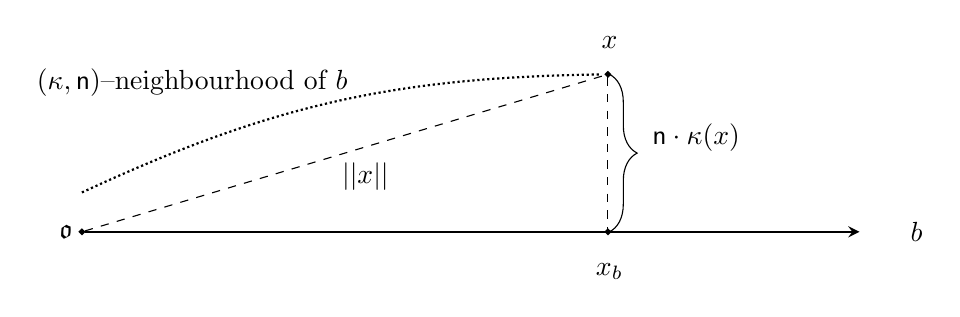
\begin{tikzpicture}
 \tikzstyle{vertex} =[circle,draw,fill=black,thick, inner sep=0pt,minimum size=.5 mm] 
[thick, 
    scale=1,
    vertex/.style={circle,draw,fill=black,thick,
                   inner sep=0pt,minimum size= .5 mm},
                  
      trans/.style={thick,->, shorten >=6pt,shorten <=6pt,>=stealth},
   ]

 \node[vertex] (a) at (0,0) {};
 \node at (-0.2,0) {$\go$};
 \node (b) at (10, 0) {};
 \node at (10.6, 0) {$b$};
 \node (c) at (6.7, 2) {};
 \node[vertex] (d) at (6.68,2) {};
 \node at (6.7, 2.4){$x$};
 \node[vertex] (e) at (6.68,0) {};
 \node at (6.7, -0.5){$x_{b}$};
 \draw [-,dashed](d)--(e);
 \draw [-,dashed](a)--(d);
 \draw [decorate,decoration={brace,amplitude=10pt},xshift=0pt,yshift=0pt]
  (6.7,2) -- (6.7,0)  node [black,midway,xshift=0pt,yshift=0pt] {};

 \node at (7.8, 1.2){$\nn \cdot \kappa(x)$};
 \node at (3.6, 0.7){$||x||$};
 \draw [thick, ->](a)--(b);
 \path[thick, densely dotted](0,0.5) edge [bend left=12] (c);
\node at (1.4, 1.9){$(\kappa, \nn)$--neighbourhood of $b$};
\end{tikzpicture}
\caption{A $\kappa$-neighbourhood of a geodesic ray $b$ with multiplicative constant $\nn$.}
\end{figure}
\end{definition}

\begin{definition} [$\kappa$-Morse I, $\kappa$-Morse II] \label{D:k-morse} \label{Def:Morse} 
Let $Z \subseteq X$ be a closed set, and let $\kappa$ be a concave sublinear function. 
We say that $Z$ is \emph{$\kappa$-Morse} if one of the following equivalent (see Proposition 3.10 \cite{QRT2})  condition holds:
\begin{enumerate}

\item[I.] There exists a proper function 
$\mm_Z : \mathbb{R}^2 \to \mathbb{R}$ such that for any sublinear function $\kappa'$ 
and for any $r > 0$, there exists $R$ such that for any $(q, Q)$-quasi-geodesic ray $\beta$
with $\mm_Z(\qq, \sQ)$ small compared to $r$, if 
$$d_X(\beta_R, Z) \leq \kappa'(R)
\qquad\text{then}\qquad
\beta|_r \subset \calN_\kappa \big(Z, \mm_Z(q, Q)\big)$$
%The function $m_Z$ will be called a $\emph{Morse gauge}$ of $Z$. 


\item[II.] There is a function
\[
\mm'_Z \from \RR_+^2 \to \RR_+
\]
so that if $\beta \from [s,t] \to X$ is a $(\qq, \sQ)$--quasi-geodesic with end points 
on $Z$ then
\[
[s,t]_{\beta}  \subset \calN_{\kappa} \big(Z,  \mm'_Z(q, Q)\big). 
\]
\end{enumerate}
\end{definition} 

\begin{remark}
By taking the maximum function of $\mm_Z, \mm'_Z,$ we may and will always assume that both conditions hold for the same $\mm_Z$, which we refer to as the $\kappa$-Morse gauge. Further,
\begin{equation} 
\mm_Z(q, Q) \geq \max(q, Q). 
\end{equation} 
\end{remark}

\begin{definition} \label{weakprojection}
Let $(X, d_X)$ be a proper geodesic metric space and $Z \subseteq X$ a closed subset, and let 
$\kappa$ be a concave sublinear function. A map $\pi_{Z} \from X \to \mathcal{P}(Z)$ is a $\kappa$-\emph{projection}  if there exist constants $D_{1}, D_{2}$, depending only on $Z$ and $\kappa$, such that for any points $x \in X$ and $z \in Z$, 
\[
\diam_X(\{z \} \cup \pi_{Z}(x)) \leq D_{1} \cdot d_X(x, z) + D_{2} \cdot \kappa(||x||).
\]
\end{definition}

A $\kappa$-projection differs from a nearest point projection by a uniform multiplicative error and a sublinear additive error. In particular, the nearest point projection is a $\kappa$-projection. Indeed, for $z \in Z$ and $w \in \pi_Z(x)$, we have
\[
d(z, w) \leq d(z, x) + d(x, w) \leq 2d(z, x).
\]
\begin{definition}[$\kappa$-weakly contracting] \label{Def:generalContracting}
For a closed subspace $Z$ of a metric space $(X, d_X)$ and a $\kappa$-projection $\pi_Z$ onto $Z$, 
we say $Z$ is \emph{$\kappa$-weakly contracting} with respect to $\pi_Z$ if there are constants $C_{1}, C_{2}$, depending only on $Z$ and $\kappa$, such that, for every 
$x,y \in X$
\[
d_X(x, y) \leq C_{1} \cdot d_X( x, Z) \quad \Longrightarrow \quad
\diam_X \big( \pi_Z(x) \cup  \pi_Z(y)  \big) \leq c_{2} \cdot \kappa(||x||).
\]
\end{definition} 
In the special case that $\pi_Z$ is the nearest point projection and $C_1 = 1$, this property was called $\kappa$\emph{-contracting} in \cite{QRT1}. It was shown in \cite{QRT1} that, in the setting of CAT(0) spaces, this is stronger than the $\kappa$-Morse condition.
\begin{proposition}\cite[Proposition A.6.]{QRT2}\label{contracting}
Let $(X, \go)$ be a proper geodesic metric space with a fixed base point and let $\alpha$ be a quasi-geodesic
ray in $X$. Let $\pi$ be any $\kappa$-projection from $X$ to $\alpha$ in the sense of Definition~\ref{weakprojection}.
Then if $\alpha$ is $\kappa$-weakly Morse, then it is $\kappa'$-weakly contracting with respect to $\pi$ for some sublinear function $\kappa'$.
\end{proposition}


\begin{definition}[$\kappa$--equivalence classes in $\pka X$] \label{Def:Fellow-Travel}
Let $\beta$ and $\gamma$ be two quasi-geodesic rays in $X$. If $\beta$ is in some 
$\kappa$--neighborhood of $\gamma$ and $\gamma$ is in some 
$\kappa$--neighborhood of $\beta$, we say that $\beta$ and $\gamma$ 
\emph{$\kappa$--fellow travel} each other. This defines an equivalence
relation on the set of quasi-geodesic rays in $X$ (to obtain transitivity, one needs to change $\nn$ of the associated $(\kappa, \nn)$--neighborhood). 
\end{definition}

We denote the equivalence class 
that contains $\beta$ by $[\beta]$:
\begin{definition}[Sublinearly Morse boundary]
Let $\kappa$ be a sublinear function as specified in Section~\ref{subfunction} and let $X$ be a \CAT space.
\[\pka X : = \{ \text{ all } \kappa\text{-Morse quasi-geodesics } \} / \kappa\text{-fellow traveling}\]
%We define the topology of $\pka X$ in Section~\ref{coarsetop}.
\end{definition}


\begin{comment}
\subsubsection{Coarse cone topology on $\pka X$}\label{coarsetop}


 We equip $\partial_\kappa X$ with a topology which is 
a coarse version of the visual topology. In visual topology, if two geodesic rays fellow travel for a long time, then they are ``close''. In this coarse version, if two geodesic rays and all the quasi-geodesic rays in their respect equivalence classes remain close for a long time, then they are close. Now we define it formally. First, we say a quantity $\sD$ \emph{is small compared to a radius $\rr>0$} if 
\begin{equation} \label{Eq:Small} 
\sD \leq \frac{\rr}{2\kappa(\rr)}. 
\end{equation} 


Recall that given a $\kappa$--Morse quasi-geodesic ray $\beta$, we denote its associated $kappa$-Morse gauge  $\mm_{\beta}(\qq, \sQ)$. These are multiplicative constants that give the heights of the $\kappa$--neighbourhoods.
\begin{definition}[topology on $\pka X$]\label{openset}
Let $\bfa \in \partial_\kappa X$ and $\alpha_0 \in \bfa$ be 
the unique geodesic in the class $\bfa$. Define$ \calU_{\kappa}(\bfa, \rr)$ to be the set of points $\bfb$ such that for any $(\qq, \sQ)$-quasi-geodesic of $\bfb$, denoted  $\beta$, 
such that $\mm_{\beta}(\qq, \sQ)$ is small compared to $\rr$, satisfies 
\[
\beta|_{\rr} \subset \calN_{\kappa}\big(\alpha_{0}, \mm_{\alpha_{0}}(\qq, \sQ)\big).\]

Let the topology of $\pka X$ be the topology induced by this neighbourhood system. The following fact shows that a $\kappa$-boundary is well defined with respect the associated group.
\end{definition}

\begin{figure}[H]
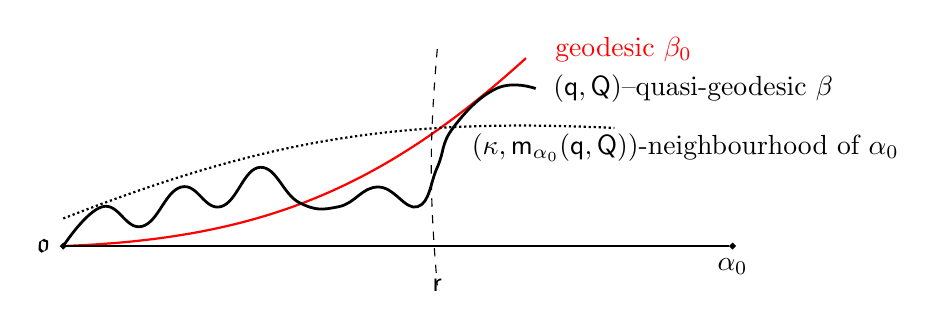
\begin{tikzpicture}[scale=0.5]
 \tikzstyle{vertex} =[circle,draw,fill=black,thick, inner sep=0pt,minimum size=.5 mm]
 
[thick, 
    scale=1,
    vertex/.style={circle,draw,fill=black,thick,
                   inner sep=0pt,minimum size= .5 mm},
                  
      trans/.style={thick,->, shorten >=6pt,shorten <=6pt,>=stealth},
   ]

  \node[vertex] (o) at (-10,0)  [label=left:$\go$] {}; 
  \node (o1) at (2, 5)[label=right:\color{red} geodesic $\beta_{0}$] {}; 
  \draw[thick, red]  (o) to [ bend right=20] (o1){};
  \node[vertex] (a) at (7,0)  [label=below:$\alpha_{0}$] {};
 \path[thick, densely dotted](-10,0.7) edge [bend left=12] (4, 3){};
 \node at (5.8, 2.5){$(\kappa, \mm_{\alpha_{0}}(\qq, \sQ))$-neighbourhood of $\alpha_{0}$};

       \node (a1) at (-1, 5) {}; 
   \node at (6,4) { $(\qq, \sQ)$--quasi-geodesic $\beta$};  
  \draw[dashed]  (-0.5, 5) to  [bend right=5] (-0.5, -1){};
  \node at (-0.5, -1){$\rr$};
 %   \draw[dashed](b)--(c){};$\rr$
   %     \draw[dashed](b)--(d){};

   \draw[thick]  (o)--(a){};
  
       
  \pgfsetlinewidth{1pt}
  \pgfsetplottension{.75}
  \pgfplothandlercurveto
  \pgfplotstreamstart
  \pgfplotstreampoint{\pgfpoint{-10cm}{0cm}}  
  \pgfplotstreampoint{\pgfpoint{-9cm}{1cm}}   
  \pgfplotstreampoint{\pgfpoint{-8cm}{0.5cm}}
  \pgfplotstreampoint{\pgfpoint{-7cm}{1.5cm}}
  \pgfplotstreampoint{\pgfpoint{-6cm}{1cm}}
  \pgfplotstreampoint{\pgfpoint{-5cm}{2cm}}
  \pgfplotstreampoint{\pgfpoint{-4cm}{1.1cm}}
  \pgfplotstreampoint{\pgfpoint{-3cm}{1cm}}
  \pgfplotstreampoint{\pgfpoint{-2cm}{1.5cm}}
  \pgfplotstreampoint{\pgfpoint{-1cm}{1cm}}
    \pgfplotstreampoint{\pgfpoint{-0.5cm}{2cm}}
      \pgfplotstreampoint{\pgfpoint{-0.1cm}{3cm}}
        \pgfplotstreampoint{\pgfpoint{1cm}{4cm}}
          \pgfplotstreampoint{\pgfpoint{2cm}{4cm}}
  %\pgfplotstreampoint{\pgfpoint{5cm}{7cm}}
  \pgfplotstreamend 
  \pgfusepath{stroke}
       
  \end{tikzpicture}
 
  \caption{ $\bfb \in \calU_{\kappa}(\bfa, \rr)$ because the quasi-geodesics of $\bfb$ such as $\beta, \beta_{0}$ stay inside the associated $(\kappa, \mm_{\alpha_{0}}(\qq, \sQ))$-neighborhood of $\alpha_{0}$ (as in Definition~\ref{Def:Neighborhood} ), up to distance $\rr$. }
 \end{figure}









\end{comment}




\begin{theorem} [\cite{QRT2}]
Let $X, Y$ be a proper metric space and let $\kappa$ be a sublinear function. The $\kappa$--boundaries of $X, Y$ are denoted $\pka X, \pka Y$. Any quasi-isometry from $X$ to $Y$ induces a homeomorphism between $\pka X$ and $\pka Y$.
\end{theorem}


%%%%%%%%%%%%%%%%%%%%%%%%%%%%%%%%%%%%%%%%%%%%%%%%%%old stuff



\subsection{First passage percolation} \label{sec23}
 $(X,d)$ be a connected graph with vertex set $V$ and edge set $E$ with the graph distance metric $d$. For a fix vertex $\mathfrak{0}, d(\gamma, \mathfrak{o})$ denote the set distance between $\mathfrak{o}$ and the set of vertices $\{\gamma(0), \gamma(1), \ldots\}$. \newline 
 Fix a probability measure $\nu$ supported on  $[0, \infty)$ and consider the product probability space
\[
\Omega = [0, \infty)^E, \quad \mathbb{P} = \nu^{\otimes E}.
\]
A typical element of $(\Omega, \mathbb{P})$ will be denoted by $\omega = \{\omega(e)\}_{e\in E}$. We define i.i.d random variables $X_e:\Omega \rightarrow [0, \infty)$ as $ X_e(\omega) = \omega(e) $ with law $\nu$. Assume $\nu(\{0\})=0.$
Assigning  $\omega(e)$ as the length of edge $e$ defines a random metric (a priori, a pseudometric) on $X$, known as the first passage percolation (FPP) metric. The metric is defined as follows:
\begin{definition}

Let $\gamma = \{e_1, \dots, e_k\}$ be an edge path. For $\omega \in \Omega$, the $\omega$- length of $\gamma$ is defined as, 
\[
|\gamma|_{\omega}  = \sum_{e \in \gamma} \omega(e)
\]
The FPP distance is defined by, 
\[
d_\omega(x, y) = \inf_\gamma |\gamma|_\omega
\]
where the infimum is over all paths $\gamma$ with terminal vertices $x$ and $y$.
    
\end{definition}
A path realizing $d_\omega(x, y)$ is called a \emph{\( \omega \)}-geodesic. 
\begin{proposition}\label{prop2.13}     \cite[Lemma 2.3, Lemma 2.5]{BT17} 
\begin{enumerate}
\item Let $X$ be a connected graph, and let $\gamma$ be a self avoiding path. Assume $0<b=\mathbb{E} \omega_{e}<\infty$. Then for a.e. $\omega$, there exists $r_{0}=r_{0}(\omega)$ such that for all $i \leq 0 \leq j$,

$$
|\gamma([i, j])|_{\omega} \leq 2 b(j-i)+r_{0}
$$
\item \label{extension} Let $X$ be an infinite connected graph with bounded degree, and let $o$ be some vertex of $X$. Assume $\nu(\{0\})=0$. Then there exists $c>0$ such that for a.e. $\omega$, there exists $r_{1}=r_{1}(\omega)$ such that for all finite path $\gamma$ such that $d(\gamma, o) \leq |\gamma|$, one has

\[|\gamma|_{\omega} \geq c|\gamma|-r_{1}\]
\end{enumerate}
\end{proposition}
\section{middle-recurrence of sublinear lines}
The idea of middle-recurrence as a characterization for Morse geodesics was first introduced by Drutu-Mozes-Sapir in \cite{DMS} and then further studied by \cite{ADT}. The characterization smartly circumvents the need for quasi-geodesic segments which renders it ideal for the application of first passage percolations. In this section, we follow the general idea of the proof of these papers and generalize the result analogously to sublinearly Morse quasi-geodesic rays.
\begin{definition}
A path in a metric space $X$ is a continuous function $p: I\rightarrow X$ from an interval $I$ to $X$. A simple path is a path that is injective. We sometimes call it a self-avoiding path in a graph, as it never visits the same vertex twice. \newline
If $p$ is any finite path in $X$, let $|p|$ denote the distance between its endpoints, and let $\ell(p)$ denote its arc length. Then the slope of $p$ is defined as:
%to be the ratio 
\[
sl(p) = \frac{\ell(p)}{|p|}
\]

\end{definition}
\begin{definition}

 For a path $\gamma$, if $a,b \in \gamma$ then  $\gamma_{[a,b]}$ the set of $x \in \gamma$ lying between $a$ and $b$. The middle third of $\gamma_{[a,b]}$ is defined as follows: \[ \gamma_{\frac{1}{3}[a,b]} := \biggl\{x\in \gamma : \min \{d(x,a),d(x,b)\} \ge \frac{1}{3}\cdot d(a,b)\biggr\}\]   


\end{definition}
\begin{definition}[$\frac{1}{3}$-middle recurrence]
    We say that a path (geodesic line or quasi-geodesic) $\beta$ is $\frac{1}{3}$-middle recurrent if for every $C\geq1$ there is a constant $c$ (depends on $C$ and $\beta$) such that the following holds:
    for any path $p$ with endpoints $a,b \in \beta$ satisfying $\ell(p)\leq Cd(a,b)$, intersects the $c\cdot \kappa$-neighborhood of the middle third of $\beta[a,b]$ for some sublinear function $\kappa$. That is,
\[ p \cap \calN_{\kappa} (\beta_{\frac 13[a,b]}, c )\neq \emptyset.\]
\end{definition}
\begin{lemma}\cite[Lemma 3.3]{ADT}\label{lemma33}
Let $\beta$ be a $\kappa'$–radius–contracting quasi-geodesic and suppose that $p$ is a path (of slope $D$) at distance
at least $K$  from $\beta$ whose endpoints have distance exactly $K$ from $\beta$. Let $|p|$ denote the distance between the endpoints of $p$. Let $s, e$ be the endpoints of $p$. Then
\[ \frac{\kappa'(K)}{2K} \geq \frac{1-(2K+\kappa'(K))/d(s, e)}{sl(p)}\]
\end{lemma}


\begin{proposition}[$\kappa$-Morse implies middle recurrence] \label{prop3.5}
Let $\beta$ be a bi-infinite geodesic line. Assume that  $\beta$ is $\kappa$-Morse with Morse gauge $m_\beta(q, Q)$. Let $p$ be any simple path with endpoints $a, b \in \beta$ and such that $\ell(p) < C d(a, b)$. Then there exists a $\kappa'$-sublinear neighborhood of $\beta$, where $\kappa'$ is the contracting function of $\beta$, and whose multiplicative constant $c(C, \beta)$ depending only on $\beta$ and $C$ such that 
\[ p \cap \mathcal{N}_{\kappa'} (\beta_{\frac 13[a,b]}, c(C, \beta)) \neq \emptyset.\]

\end{proposition}
\begin{proof}
    To proceed, let 
    $\kappa'$ denote the contracting function of $\beta$ of Proposition~\ref{contracting}. By way of contradiction, suppose there does not exist any sublinear neighborhood of $\beta$ in which $p$ intersects the middle third. We first define a \emph{linear neighborhood} with constant $c$:
     
  \[Ln(\beta, c) : = \{ x \in X | \, d(x, \beta) \leq c \cdot d(\go, x)\}.\]
  The assumption implies that there exists a constant $c_1(C)$ such that there exists a family of paths $\{p_i \}$ with slope at most $C$ such that for arbitrarily large $t$, there exists a $p_i$ and $t$ such that  $p_i(t)$ is outside of the $c_1$-linear neighborhood of the middle third of the geodesic segment connecting the endpoints of $p_i$ (which we denote $s_i$ and $e_i$). Without loss of generality we can assume $0<c_1 <1.$ Moreover, we can assume that 
  \[d(s_i, \go) \geq i.\]
  Since the path $p_i$ is chosen to traverse outside of the $Ln(\beta, c_1),$ we can assume without loss of generality that eventually there exists a constant $c_3$ such that 
  \[
  d(e_i, \go) \geq c_3 d(s_i, \go).
  \]
  
  
  Given any such $p_i$, let $p_i'$ be a connected segment of $p_i$ that is outside the $c_1$-linear neighborhood of $\beta$ and does not intersect the $c_1$-linear neighborhood of the middle third. The endpoints of $p'_i$ we denote $s'_i$ and $e'_i$.
  
  Since $\beta$ is $\kappa'$-contracting with respect to distance from the base point. For any ball $B$ disjoint from $\beta$ and centered at a point $x \in p'_i$, 
  \begin{equation}\label{contractingball}
  \diam(\pi_\beta(B)) < c_2 \kappa'(d(x, \go)).
  \end{equation}
  Since $x \in p'_i$ is outside of the $c_1$-linear neighborhood, we have that
  \[ c_1 d(x, \go) \leq d(x, \beta)  \]
  thus we have
  \[\diam(\pi_\beta(B)) < c_2 \kappa'(d(x, \go))
\leq c_2 \kappa'(\frac{1} {c_1} d(x, \beta))\leq \frac{c_2}{c_1} \kappa'(d(x, \beta)).\]
Thus, such balls are $\kappa'$-radius-contracting with constant $c_2/c_1$. Thus we have proven the following claim:
\begin{claim}\label{radial-contracting}
Let $\beta$ be a sublinearly Morse geodesic line that is 
$\kappa'$-contracting in the sense of Definition~\ref{Def:generalContracting} with constant $c_2$. Then any ball disjoint from $\beta$ and whose center is outside of the $c_1$-linear-neighborhood of $\beta$ has $\kappa'$-radius-contracting property with constant $\frac{c_2}{c_1}$.
\end{claim}

%------------draft piture--------------------------
\begin{figure}
    \centering
\tikzset{every picture/.style={line width=0.75pt}} %set default line width to 0.75pt        

\begin{tikzpicture}[x=0.75pt,y=0.75pt,yscale=-1,xscale=1]

%Straight Lines [id:da8955665966371212] 
\draw    (50.24,164.76) -- (11.86,164.76) ;
\draw [shift={(9.86,164.76)}, rotate = 360] [color={rgb, 255:red, 0; green, 0; blue, 0 }  ][line width=0.75]    (10.93,-3.29) .. controls (6.95,-1.4) and (3.31,-0.3) .. (0,0) .. controls (3.31,0.3) and (6.95,1.4) .. (10.93,3.29)   ;
%Straight Lines [id:da8806859470582984] 
\draw  [dash pattern={on 0.84pt off 2.51pt}]  (124.62,124.12) -- (399.75,68.51) ;
%Curve Lines [id:da8724418300710257] 
\draw [color={rgb, 255:red, 139; green, 87; blue, 42 }  ,draw opacity=1 ]   (264.25,52.92) .. controls (312.43,49.39) and (255.73,79.26) .. (301.61,87.02) ;
%Curve Lines [id:da6064520648832785] 
\draw [color={rgb, 255:red, 139; green, 87; blue, 42 }  ,draw opacity=1 ]   (180.9,111.49) .. controls (222.96,-57.87) and (221.43,47.98) .. (264.25,52.92) ;
%Curve Lines [id:da3510889648758053] 
\draw    (301.61,87.02) .. controls (339.84,94.78) and (366.72,165.12) .. (398.07,166.53) ;
%Curve Lines [id:da9434371861660892] 
\draw    (68.49,164.76) .. controls (129.66,122.42) and (119.72,153.83) .. (180.9,111.49) ;
%Shape: Arc [id:dp27205301504729806] 
\draw  [draw opacity=0][dash pattern={on 4.5pt off 4.5pt}] (203.67,165) .. controls (201.2,156.72) and (197.36,146.41) .. (192.37,135.1) .. controls (188.42,126.14) and (184.23,117.61) .. (180.13,110.06) -- (181.27,132.81) -- cycle ; \draw  [dash pattern={on 4.5pt off 4.5pt}] (203.67,165) .. controls (201.2,156.72) and (197.36,146.41) .. (192.37,135.1) .. controls (188.42,126.14) and (184.23,117.61) .. (180.13,110.06) ;  
%Shape: Arc [id:dp7753120026034933] 
\draw  [draw opacity=0][dash pattern={on 4.5pt off 4.5pt}] (310.53,161.91) .. controls (312.21,155.03) and (310.32,133) .. (305.43,106.07) .. controls (304.16,99.08) and (302.79,92.31) .. (301.37,85.96) -- (297.56,103.19) -- cycle ; \draw  [dash pattern={on 4.5pt off 4.5pt}] (310.53,161.91) .. controls (312.21,155.03) and (310.32,133) .. (305.43,106.07) .. controls (304.16,99.08) and (302.79,92.31) .. (301.37,85.96) ;  
%Flowchart: Connector [id:dp7901950746928997] 
\draw   (156.18,106.7) .. controls (156.18,94.32) and (167.02,84.28) .. (180.39,84.28) .. controls (193.76,84.28) and (204.6,94.32) .. (204.6,106.7) .. controls (204.6,119.09) and (193.76,129.13) .. (180.39,129.13) .. controls (167.02,129.13) and (156.18,119.09) .. (156.18,106.7) -- cycle ;
%Shape: Parabola [id:dp9579653486386642] 
\draw   (222.97,166.06) .. controls (217.86,139.31) and (210.72,115.71) .. (201.54,95.27) ;
%Shape: Parabola [id:dp5596465562476505] 
\draw   (161.81,119.68) .. controls (167.14,135.68) and (172.96,150.75) .. (179.28,164.92) ;
%Shape: Brace [id:dp3353591586819993] 
\draw   (184.72,170.17) .. controls (184.81,174.84) and (187.19,177.12) .. (191.86,177.03) -- (192.45,177.02) .. controls (199.12,176.89) and (202.5,179.15) .. (202.59,183.82) .. controls (202.5,179.15) and (205.78,176.75) .. (212.45,176.62)(209.45,176.68) -- (213.04,176.61) .. controls (217.71,176.52) and (219.99,174.14) .. (219.9,169.47) ;
%Straight Lines [id:da683589745854115] 
\draw    (9.86,164.76) -- (421,167.01) ;
\draw [shift={(423,167.02)}, rotate = 180.31] [color={rgb, 255:red, 0; green, 0; blue, 0 }  ][line width=0.75]    (10.93,-3.29) .. controls (6.95,-1.4) and (3.31,-0.3) .. (0,0) .. controls (3.31,0.3) and (6.95,1.4) .. (10.93,3.29)   ;

% Text Node
\draw (63.75,170.25) node [anchor=north west][inner sep=0.75pt]  [font=\scriptsize]  {$s_{i}$};
% Text Node
\draw (390.74,169.26) node [anchor=north west][inner sep=0.75pt]  [font=\scriptsize]  {$e_{i}$};
% Text Node
\draw (172.34,98.66) node [anchor=north west][inner sep=0.75pt]  [font=\tiny,color={rgb, 255:red, 208; green, 2; blue, 27 }  ,opacity=1 ]  {$s_{i} '$};
% Text Node
\draw (299.79,74.43) node [anchor=north west][inner sep=0.75pt]  [font=\tiny,color={rgb, 255:red, 208; green, 2; blue, 27 }  ,opacity=1 ]  {$e_{i} '$};
% Text Node
\draw (208.1,154.53) node [anchor=north west][inner sep=0.75pt]  [font=\tiny,color={rgb, 255:red, 208; green, 2; blue, 27 }  ,opacity=1 ]  {$x$};
% Text Node
\draw (321.3,153.21) node [anchor=north west][inner sep=0.75pt]  [font=\tiny,color={rgb, 255:red, 208; green, 2; blue, 27 }  ,opacity=1 ]  {$y$};
% Text Node
\draw (5.63,169.15) node [anchor=north west][inner sep=0.75pt]  [font=\scriptsize]  {$\mathfrak{o} $};
% Text Node
\draw (194.36,128.86) node [anchor=north west][inner sep=0.75pt]  [font=\tiny]  {$K_{i}$};
% Text Node
\draw (186.74,178.42) node [anchor=north west][inner sep=0.75pt]  [font=\tiny,xslant=0.01]  {$\frac{c_{2}}{c_{1}} \ \kappa '( K_{i})$};
% Text Node
\draw (227.09,86.1) node [anchor=north west][inner sep=0.75pt]  [font=\tiny,color={rgb, 255:red, 126; green, 211; blue, 33 }  ,opacity=1 ,rotate=-347.06]  {$c_{3} K_{i}$};
% Text Node
\draw (245.14,27.53) node [anchor=north west][inner sep=0.75pt]  [font=\tiny]  {$p_{i} '$};
% Text Node
\draw (361.35,82.19) node [anchor=north west][inner sep=0.75pt]  [font=\tiny,xslant=0.27]  {$Ln( c_{1} ,\beta )$};
% Text Node
\draw (263.95,39.38) node [anchor=north west][inner sep=0.75pt]  [font=\tiny,color={rgb, 255:red, 139; green, 87; blue, 42 }  ,opacity=1 ]  {$sl( p_{i} ') \leq 3CK$};
% Text Node
\draw (351.28,110.42) node [anchor=north west][inner sep=0.75pt]  [font=\tiny]  {$p_{i}$};
% Text Node
\draw (363.73,124.06) node [anchor=north west][inner sep=0.75pt]  [font=\tiny]  {$sl( p_{i}) \leq C$};


\end{tikzpicture}
  \caption{Behavior of the path outside $c_1$-linear neighborhood of $\kappa$-Morse geodesic line $\beta$.}
    \label{fig:enter-label}
\end{figure}
Secondly, suppose the end points of $p_i'$ are $(s'_i, e'_i)$. 
  and we know that by construction \[
  d(s_i, e_i) = c_3 d(s_i, \go).
  \]
  By construction there exists points $x, y \in \beta$ such that
  \[d(x, s_i') = c_1 d(\go, s_i') \,\text{ and }\, d(y, e_i') = c_1 d(\go, e_i')\]
  Now estimate,
 \begin{align*}
 d(\go,s_i')
 &\leq d(x,\go)+d(x,s_i')\\
 &\leq d(s_i,\go)+\frac{c_3-1}{3}d(s_i,\go)+d(s_i',\go)
 \end{align*} implies,
 \[(1-c_1)d(\go,s_i')\leq  \bigg(\frac{c_3-1}{3} +1\bigg)d(s_i, \go)\]
 Hence,
 \begin{equation}\label{estimate1}
   d(x,e_i')\leq \frac{c_1}{1-c_1} \bigg(\frac{c_3-1}{3} +1\bigg)d(s_i, \go)
   \end{equation}
Similarly we have,
\begin{equation}\label{estimate2}
 d(y,e_i')\leq \frac{c_1}{1-c_1} \bigg(\frac{2(c_3-1)}{3} +1\bigg)d(s_i, \go)   
\end{equation}   
 By the generalized triangle inequality and using estimate~\ref{estimate1} and ~\ref{estimate2} we have, 
 \begin{align*}
   d(s'_i, e'_i) 
   &\geq d(x, y) -\frac{c_1}{1-c_1} \bigg(\frac{c_3-1}{3} +1\bigg)d(s_i, \go)- \frac{c_1}{1-c_1} \bigg(\frac{2(c_3-1)}{3} +1\bigg)d(s_i, \go)\\
   & \geq \frac{1}{3}d(s_i,e_i)-\frac{c_1}{1-c_1}\frac{c_3+1}{c_3-1}d(s_i,e_i)\\
   & \geq \frac{1}{3} \cdot \frac{1}{K}\cdot d(s_i,e_i), \ \  \ \text{where}\ \frac{1}{K} :=1- \frac{c_1}{3(1-c_1)}\frac{c_3+1}{c_3-1}.
 \end{align*}
 We can choose $c_3$ large enough compared to $c_1$ so that $K$ is uniformly bounded above. 
  Thus 
  \[ sl(p'_i) = \frac{|p'_i|}{d(s'_i, e'_i)} \leq \frac{|p'_i|}{\frac{1}{3K}d(s_i, e_i)} \leq
   \frac{|p_i|}{\frac{1}{3K}d(s_i, e_i)} = 3KC.\]
   
 
%---------previous work/details---
\begin{comment}
 Secondly, suppose the end points of $p_i'$ are $(s'_i, e'_i)$. 
  and we know that by construction \[
  d(s_i, e_i) = c_3 d(s_i, \go).
  \]
  By construction there exists points $x, y \in \beta$ such that
  \[d(x, s_i') = c_1 d(\go, s_i') \,\text{ and }\, d(y, e_i') = c_1 d(\go, e_i')\]


  By the generalized triangle inequality, we have that 
  \[ d(s'_i, e'_i) \geq d(x, y) -c_1 (\frac{c_3-1}{3} +1)d(s_i, \go)-
  c_1 (\frac{2(c_3-1)}{3} +1)d(s_i, \go).\]


  Thus
  \[ d(s'_i, e'_i) \geq  c_1( d(\go, e_i') -d(\go, s_i'))= c_1 d(x, y) \geq   \frac 13 c_1 d(s_i, e_i)\]
  Thus 
  \[ sl(p'_i) = \frac{|p'_i|}{d(s'_i, e'_i)} \leq \frac{|p'_i|}{\frac 13 c_1 d(s_i, e_i)} \leq
   \frac{|p_i|}{\frac 13 c_1 d(s_i, e_i)} = 3 c_1 C.\]
    
\end{comment}
   
Furthermore, we claim that for large enough $i$, 
  $d(s_i, e_i)$ does not grow sublinearly with respect to 
  $d( \go, s_i)$: otherwise, since slope of $p_i$ are bounded, eventually $p_i$ will not be outside of the linear neighborhood of $\beta$, thus there exists a constant $c_2>0$ where
  \[
   d(s_i, e_i) \geq c_2 d(\go, s_i).
  \]
  Let $K_i:= d(s'_i, \beta)$. A slight adaptation of the Lemma~\ref{lemma33} yields 
  %---ADT lemma after adjusting all the constants--------
   \[ \frac{\kappa'(K_i)}{K_i} \geq \frac{6c_1C-(2 K_i +c_2'\kappa'(K_i))/d(s'_i, e'_i)}{c_2'(3KC+1)}\]
   Where $c_2'=\frac{c_2}{c_1}$ from claim ~\ref{contractingball}.\newline
   As we argued before,  as $i \to \infty$,  $d(s'_i, e'_i)$ grows linearly with respect to $d(s_i, e_i)$ and hence $K_i$. Thus by construction, there exists $c_4$ such that for all $i$ large enough, $d(s'_i, e'_i) \geq c_4 K_i$ and since $\lim_{t\to\infty}\frac{\kappa'(t)}{t}=0$, there exists a uniform constant $D>0$ depending only on $C, c_1, c_2, c_3,c_4, \kappa, \kappa'$ where 
  \[
  \frac{6c_1C-(2 K_i +c_2'\kappa'(K_i))/c_4K_i}{c_2'(3KC+1)}\geq D.
  \]
 
 % previous one without adjustment of constant----
   \begin{comment}
   \[ \frac{\kappa'(K_i)}{K_i} \geq \frac{1-(c_2' K_i +\kappa(K_i))/d(s'_i, e'_i)}{3KC}\]
  As we argued before,  as $i \to \infty$,  $d(s'_i, e'_i)$ grows linearly with respect to $d(s_i, e_i)$ and hence $K_i$. Thus by construction, there exists $c_4$ such that for all $i$ large enough, $d(s'_i, e'_i) \geq c_4 K_i$ and since $\lim_{t\to\infty}\frac{\kappa(t)}{t}=0$, there exists a uniform constant $D>0$ depending only on $C, c_1, c_2, c_3,c_4, \kappa, \kappa'$ where 
  \[
  \frac{1-(c'_2 K_i +\kappa(K_i))/c_4 K_i}{3KC} \geq D.
  \]
\end{comment}
%----------  
  Thus, we have that
  \[\frac{\kappa'(K_i)}{K_i} \geq D
\]
  There exists a maximal $K_i$ for which the inequality holds, which is a contradiction as desired. 

\end{proof}

\begin{comment}
    

\begin{itemize}
\item  the length of $L(\p)\leq Cd(a,b)$
\item ${\kappa(|b|)< \frac{e|b|}{6M(C,0)[2+M(C,0)A]}}$.
\item $d(a,b)\geq e|b|$ for some constant $A$.
\end{itemize}
Then for every $C\geq 1$ and $e > 0$ there exists $D=D(C)$ such all such segments $p$ intersect the $D\cdot\kappa$-neighborhood of the middle third of the segment $[a, b]_\beta$
%\end{proposition}


%below is old stuff
We first demonstrate an interesting property of sublinearly Morse quasi-geodesics.

\begin{proposition}
Let $\beta$ be a bi-infinite geodesic line. Assume that  $\beta$ is $\kappa$-Morse with Morse gauge $M$. Let $p$ be any $\qq$-quasi-geodesic segments with following properties:
\begin{itemize}
\item  the length of $L(\p)\leq Cd(a,b)$
\item ${\kappa(|b|)< \frac{e|b|}{6M(C,0)[2+M(C,0)A]}}$.
\item $d(a,b)\geq e|b|$ for some constant $A$.
\end{itemize}
Then for every $C\geq 1$ and $e > 0$ there exists $D=D(C)$ such all such segments $p$ intersect the $D\cdot\kappa$-neighborhood of the middle third of the segment $[a, b]_\beta$
\end{proposition}
    
\begin{proof}
    Suppose $\beta$ is a $\kappa$-Morse geodesic ray starting at $\mathfrak{o}$ with Morse gauge function $M:\mathbb{R}^2 \rightarrow \mathbb{R}$. For $\kappa$ being sublinear there exist a $t$ such that 
    \[M(C,0)\kappa(t)< e\cdot t.\] Now, by way of contradiction, for some fixed $C\geq 1$ and $D(C)>0$ there exist a $C$- biLipschitz path $\p:[0,L]\rightarrow X$ joining $a,b$ with $L \leq Cd(a,b)$, for which \[\p \cap N_\kappa(\frac{1}{3}\beta[r,s], D(C))= \phi.\]  Moreover, $\beta$ is $\kappa$-Morse hence, $\p \subset N_\kappa(\beta, M(C,0))$.  
    
    
    There are two cases to consider:\newline
    \textit{Case 1.} Let $\p \cap N_\kappa(\frac{1}{3}\beta[r,s], M(C,0))= \phi $, then for every $c \in \p$ there exists a point $\eta_c\in \beta $ such that $d(c,\eta_c)\leq M(C,0)\kappa(|c|)$, where $\eta_c$ is either in $\beta_l$ and $\beta_r$, where \[\beta_l=\{x \in \beta : d(x,a)\leq \frac{1}{3}d(a,b) \text{ or } x\in [\mathfrak{o},a]_{\beta}\}\]
    and \[\beta_r= \{x \in \beta : d(y,b)\leq \frac{1}{3}d(a,b)\]
     or \[ y\in [b,\infty]_{\beta} \}.\] If the whole path is in $\kappa$- neighborhood of either $\beta_l$ or $\beta_r$ then \[d(a,b) \leq M(C,0)\kappa(|a|)+M(C,0)\kappa(|b|)< e|b|\]
     which is a contradiction. Every point on $\p$ is $M(C,0)\cdot \kappa$-close to either $\beta_l$ or $\beta_r$.
\begin{claim}There exists a $\eta$ such that \[d(\eta,\beta_l)\leq M(C,0)\kappa(|\eta|) \text{ and } d(\eta,\beta_r)\leq M(C,0)\kappa(|\eta|).\] 
\end{claim}
\begin{proof} Suppose every point is either close to only $\beta_l$ or $\beta_r$. 
$H$ be the set of all closed sub arc of $\p$ which contains in $M\cdot\kappa$ neighborhood of $\beta_l$, and similarly $K$ be the set of all closed sub arc of $\p$ which is $M\cdot\kappa$ close to $\beta_r$.  So, $\p=H \cup K$ with$H \cap K = \phi$. Which is a contradiction to the fact that $\p$ is connected. Therefore, there is a point $\eta$ such that it is $M(C,0).\kappa$-close to both $\beta_l,\beta_r.$ \newline
If $x\in \beta_l$ and $y\in \beta_r$ then $d(x,y)\geq \frac{1}{3} d(a,b)\geq \frac{e|b|}{3}$. 
 From \textit{Claim 1} we conclude that, \[ \frac{e|b|}{3} \leq d(x,y) \leq d(\eta,x)+d(\eta,y)\leq 2 M(C,0) \kappa(|\eta|)\]
From the lemma 3.1 and the fact that $d(\eta,y)\leq M(C,0)\kappa(|\eta|)$, we can say there exists $D_1= 2+M(C,0)A$, where $A$ is a constant (depends on $\kappa$) such that $\kappa (|\eta|)\leq D_1 \kappa (|y|)$. 
\newline 
Since, $\beta$ is $\kappa$- Morse geodesic then we have,
\[\frac{e|b|}{3} \leq d(x,y) \leq 2M(C,0)(2+2M(C,0)A)\kappa(|b|)\] 
therefore,
\begin{equation} 
\begin{split}
 \frac{e|b|}{3}&\leq 2M(C,0)(2+2M(C,0)A)\kappa(|b|) \\\\
   {e|b|} &\leq 6M(C,0)(1+M(C,0)A)\kappa(|b|)\\\\
    \kappa(|b|)&\geq \frac{e|b|}{6M(C,0)[2+M(C,0)A]} 
\end{split}
\end{equation}
Which is a contradiction! Hence our assumption $\beta$ being $\kappa$-Morse is wrong.\end{proof}

\textit{Case 2.}  Let $\p \cap N_\kappa(\frac{1}{3}\beta[r,s], M(C,0)) \neq \phi $. By the way of contradiction we also have $\p \cap N_\kappa(\frac{1}{3}\beta[r,s], D(C))= \phi $. Therefore, $M(C,0) > D(C)$.
\newline Now consider the $\kappa$-neighborhood $N_\kappa(\beta, D(C))$. Suppose $\mathcal{O}$ be the set of all open sub arcs which are outside of $N_\kappa(\beta, D(C))$. 
 The last time, when it enters the neighborhood, if the terminal points of the arc will be close to $\beta_l$ then for some $x \in \beta_l$, 
 \begin{align*}
d(b,x)&\leq D(C)\kappa(|b|)\\ 
   \frac{e|b|}{3} & \leq D(C)\kappa(|b|)\\
   \frac{e|b|}{3}&< \frac{e|b|\cdot D(C)}{6M(C,0)[2+2M(C,0)A]}
 \end{align*}
 After simplifying above we will get $M(C,0)\cdot A < 0$ which can not be possible. \newline
 
 Therefore, there is a close sub arc (say, $\mathfrak{h}$) inside  $N_\kappa(\beta, D(C))$ whose terminal points are close to $\beta_l$ and $\beta_r$ respectively.  The goal is to use the \textit{case 1} for this close sub arc $\mathfrak{h}$ in $\mathcal{O}^c$. Similarly like case 1, $H$ be the set of all closed sub arc of $\mathfrak{h}$ which contains in $D(C)\cdot\kappa$ neighborhood of $\beta_l$, and $K$ be the set of all closed sub arc of $\mathfrak{h}$ which is $D(C)\cdot\kappa$ close to $\beta_r$. $H\cup K= \mathfrak{h}$. Hence, there is a point $\eta$ such that it is $D(C).\kappa$-close to both $\beta_l,\beta_r$ such that
 \[ d(\eta,x)\leq D(C)\kappa(|\eta|)\]
 and \[d(\eta,y)\leq D(C)\kappa(|\eta|)\]
 for some $x \in \beta_l$ and $y\in \beta_r$. Then by applying lemma 3.1 we have, \[\kappa(|\eta|)\leq (2+2D(C)A)\kappa(|x|)\leq (2+2D(C)A)\kappa(|b|).\]
Now by applying the case 1, we can conclude that\[\kappa(|b|)\geq \frac{e|b|}{6D(C)[2+2D(C)A]} \geq \frac{e|b|}{6M(0C,0)[2+M(C,0)A]}\] 
Which is a contradiction to our assumption! This complete the proof.\end{proof}






That is to say, all linearly long path is in the sublinear neighborhood. We deduce the following criterion, which we shall use in the sequel. 
\end{comment}

\begin{lemma} \label{lemma36}   
Let $X$ be an infinite connected graph with bounded degree. Assume $\gamma_{0}$ is a bi-infinite $\kappa$-Morse quasi-geodesic. Then there exists an increasing function $\phi: \mathbb{R}_{+} \rightarrow \mathbb{R}_{+}$such that $\lim _{t \rightarrow \infty} \phi(t)=\infty$, and with the following property. Assume

\begin{itemize}
  \item $x, y$ belong to $\gamma_{0}$.
  \item $x'$ and $y'$ are vertices such that $d\left(x, x'\right)=d\left(y, y'\right)=R$, and $d\left(x', y'\right) \geq 4 R$;
  \item $\gamma$ is a quasi-geodesic joining $x'$ to $y'$, and remains outside of the $R$-neighborhood of $\gamma_{0}$.
\end{itemize}
Then
\[|\gamma| \geq \phi(R) d(x, y)\]
\end{lemma}

\begin{proof} Assume by contradiction that there does not exist such a $\phi(R)$, that is, eventually for the paths $\gamma$ long enough becomes a path whose length is bounded above linearly. Then Proposition~\ref{prop3.5} implies that these paths intersect a sublinear neighborhood of the middle third with bounded constants. However, the choice of $x, y$ is such that $\gamma$ is outside of larger and larger linear neighborhoods, thus we have the desired contradiction. Now we start with the formal proof.

Suppose by contradiction that there exists a constant $C>0$, and for every $n$, consider the path $\gamma$ joining the vertices $x',y'$ with $|\gamma| \leq C\cdot d(x,y)$,  such that $d\left(x, x'\right)=d\left(y, y'\right)=R, d\left(x', y'\right) \geq 4 R$, and $\gamma$ avoids the $R$-neighborhood of $\gamma_{0}$, where $R$ is an integer greater than $d(x,y)$. By our assumption, \[4R \leq d(x',y') \leq d(x',x)+d(x,y)+d(y,y')\leq 2R + d(x,y)\]  thus, \[d(x,y) \geq 2R\] Now consider the path $p$ that is a concatenation of  $[x,x']$, $\gamma$ and $[y',y]$, then $|p| \leq 2R+ |\gamma| \leq d(x,y) + C d(x,y) \leq C'd(x,y)$, where $C'=1+C$. Then by Proposition~\ref{prop3.5} there exists a $\kappa'$-sublinear neighborhood of $\gamma_0$ where $\kappa'$ is the contracting function of $\gamma_0$ such that $p$ intersects the $c \cdot \kappa'$-neighborhood of the middle third of $\gamma_0[x,y]$, where $c$ is the multiplicative constant depends only on $\gamma_0$ and $C'.$ Suppose $p_i$ be a point which is in the intersection. Since $d(x,y)\geq R$, by choosing $d(x,y)$ large enough we can assume also $R\geq c \cdot \kappa'(d(\mathfrak{o},p_i))$. This contradicts the assumption of Lemma ~\ref{lemma36} since $\gamma$ avoids $R$- neighborhood of $\gamma_0$. 
\end{proof}


%%%%--
\begin{comment}
    

Recall from Equation~\ref{contractingball} that since $\gamma$ is  $c_2\cdot\kappa'$ sublinearly contracting and since 
\[d(x, \go) \geq ?? \]
we have that  \[ d(x,y) \leq \frac{c_2}{c_1} \kappa'(d(x', y')).\]
 By choosing $d(x,y)$ large enough, we can assume also that $R> \frac{c_2}{c_1} \cdot \kappa'$. Applying the Proposition~\ref{prop3.5}, the path $p$ will intersect the middle third neighborhood with a height $\frac{c_2}{c_1} \cdot \kappa'$. This contradicts the assumption of Lemma~\ref{lemma36}.

\end{comment}

Now we are ready to prove Theorem~\ref{introthm1}:
\begin{theorem}\label{thm38}
Let $X$ be an infinite connected graph with bounded degree. Assume $\EE \omega_e < \infty$ and $\nu(0) = 0$. If $X$ contains a sublinearly Morse bi-infinite quasi-geodesic line, then for almost every $\omega$, there is a bi-infinite geodesic ray $\gamma_\omega \subset X_\omega$. Furthermore, there exists a constant $K$ depending only on $\gamma_0 \subset X$ and $\omega$, such that
\[d_{X_\omega} (\go, \gamma_\omega) \leq K. \]
\end{theorem}
\begin{proof}
Let $\gamma_0$ be a bi-infinite $\kappa$-Morse quasi-geodesic line. By \cite[Lemma 4.2 (1)]{QRT2}, there exists a $\kappa$-Morse bi-infinite geodesic line in the neighborhood $\calN_\kappa( \gamma,m_\gamma(1,0))$. Thus without loss of generality, we can pass to a bi-infinite $\kappa$-Morse geodesic line, which we denote $\gamma_0$. Denote $\go=:\gamma_{0}(0)$. Consider two sequences of vertices $(x_{n})$ and $(y_{n})$ on $\gamma_{0}$ escaping to infinity in opposite directions such that 
\[d(x_n, \go) = n \text{ and } d(y_n, \go) = n.\]

Let $\Omega' \subset \Omega$ be a measurable subset of full measure for which Proposition ~\ref{prop2.13} holds. For all $n$ and for all $\omega$, we pick measurably an $\omega$-geodesic $\gamma_{\omega}^{n} \in X_{\omega}$ between $x_{n}$ and $y_{n}$ (these vertices are in both $X$ and $X_\omega$). 
By Proposition ~\ref{prop2.13}, we have that $d_{\omega}\left(x_{n}, y_{n}\right)$ is finite, so paths between $x_n, y_n$ of finite length whose $\omega$-length is near to $d_\omega(x_n,y_n)$. Any path between $x_n, y_n$ in $X$ has the property $d(\mathfrak{o, \gamma)\leq |\gamma|}$. Therefore by Proposition ~\ref{prop2.13} paths of length $\geq M$ have $\omega$-length going to infinity as $M \rightarrow \infty$. That is, extremely large paths must have large $\omega$-length. Therefore, the infimum of $\omega$-lengths of all such paths exists. Thus geodesic segments $\gamma_{\omega}^{n}$ exists. Furthermore,  let $\gamma^n$ denote the image of $\gamma_{\omega}^{n}$ in $X$. In fact, for an integer $i$, $\gamma^n(i)=\gamma_{\omega}^{n}(i).$
\begin{comment}
    
 we first claim
\begin{claim}
There exists $q, Q$ where all $\gamma_n$ are $(q,Q)$-quasi-geodesic segments.
\end{claim}
\begin{proof}
    Since $[x^n_\omega, \go]$ and $[y^n_\omega, \go]$ are geodesic segments where 
    ??
    Consider $i,j$ be two real numbers and $\gamma_{\omega}^{n}(i)$ and $\gamma_{\omega}^{n}(j)$
\end{proof}
\end{comment}
\newline
The proof has two parts, firstly, if we can prove that for all $\omega \in \Omega'$, there exists a constant $R_{\omega}>0$ such that for all $n, d\left(\gamma_{\omega}^{n}, \mathfrak{o}\right) \leq R_{\omega}$, then the main theorem follows by Arzelà–Ascoli theorem. So we shall assume by contradiction that for some $\omega \in \Omega'$, there exists a sequence $R_{n}$ going to infinity such that none of the vertices on the geodesic $\ga_n^\omega$ lies with in $10R_n$ graph distance from the base point $\mathfrak{0}$. 
\begin{lemma}\label{lemma38}
Assuming the above, there exist integers $p<q$ such that
\[d\left(\gamma_{\omega}^{n}(p), \gamma_{0}\right)=d\left(\gamma_{\omega}^{n}(q), \gamma_{0}\right)=R_{n}\]
and such that for all $p \leq k \leq q$,
\[
d\left(\gamma_{\omega}^{n}(k), \gamma_{0}\right) \geq R_{n}
\]and
\[
d\left(\gamma_{\omega}^{n}(p), \gamma_{\omega}^{n}(q)\right) \geq 4 R_{n}\]
\end{lemma}
\begin{proof}  Let $\gamma_{0}(i)$ and $\gamma_{0}(j)$ with $i<0<j$ be the two points at distance $10 R_{n}$ from $o=\gamma_{0}(0)$. Since $\gamma_{0}$ is a $\kappa$-Morse geodesic line, $\gamma_{0}((\infty, i])$ and $\gamma_{0}([j, \infty))$ are distance $20 R_{n}$ from one another. 

%----------------picture for the proof---------------------- %
\begin{figure}
    

\tikzset{every picture/.style={line width=0.75pt}} %set default line width to 0.75pt        

\begin{tikzpicture}[x=0.75pt,y=0.75pt,yscale=-1,xscale=1]
%uncomment if require: \path (0,300); %set diagram left start at 0, and has height of 300

%Straight Lines [id:da0728767853419866] 
\draw    (96.33,196.51) -- (682.06,193.42) ;
%Shape: Right Angle [id:dp8924284736788338] 
\draw   (248.44,173.61) -- (248.44,139.74) -- (279.17,139.74) ;
%Straight Lines [id:da14795673410618326] 
\draw  [dash pattern={on 0.84pt off 2.51pt}]  (399.55,193.86) -- (451.95,112.81) ;
%Shape: Ellipse [id:dp2884973309694271] 
\draw   (306.77,194.1) .. controls (306.77,139.29) and (349.78,94.86) .. (402.84,94.86) .. controls (455.9,94.86) and (498.91,139.29) .. (498.91,194.1) .. controls (498.91,248.9) and (455.9,293.33) .. (402.84,293.33) .. controls (349.78,293.33) and (306.77,248.9) .. (306.77,194.1) -- cycle ;
%Straight Lines [id:da052239629390981146] 
\draw    (248.44,173.61) -- (248.19,196.91) ;
%Shape: Ellipse [id:dp20268556563605444] 
\draw  [color={rgb, 255:red, 218; green, 16; blue, 40 }  ,draw opacity=1 ] (280.97,139.74) .. controls (280.97,138.71) and (280.16,137.87) .. (279.17,137.87) .. controls (278.17,137.87) and (277.36,138.71) .. (277.36,139.74) .. controls (277.36,140.77) and (278.17,141.61) .. (279.17,141.61) .. controls (280.16,141.61) and (280.97,140.77) .. (280.97,139.74) -- cycle ;
%Straight Lines [id:da7779973108377634] 
\draw [color={rgb, 255:red, 219; green, 25; blue, 25 }  ,draw opacity=1 ] [dash pattern={on 4.5pt off 4.5pt}]  (279.17,139.74) -- (279.68,196.24) ;
%Straight Lines [id:da6036674557383928] 
\draw    (278.68,82.39) -- (279.17,139.74) ;
%Shape: Right Angle [id:dp14615976314985257] 
\draw   (340,82.19) -- (387.03,82.19) -- (387.03,63.7) ;
%Shape: Right Angle [id:dp5951866533299037] 
\draw   (404.41,63.7) -- (430.48,63.7) -- (430.48,73.21) ;
%Shape: Right Angle [id:dp920119416327674] 
\draw   (430.48,73.21) -- (476.99,73.21) -- (476.99,104.89) ;
%Straight Lines [id:da7879189165417656] 
\draw    (387.03,63.7) -- (404.41,63.7) ;
%Shape: Right Angle [id:dp08222154201971255] 
\draw   (476.99,104.89) -- (511.24,104.89) -- (511.24,137.1) ;
%Shape: Right Angle [id:dp758473002205558] 
\draw   (511.24,137.1) -- (551.63,137.1) -- (551.63,193.6) ;
%Shape: Ellipse [id:dp36363907542696006] 
\draw  [color={rgb, 255:red, 218; green, 16; blue, 40 }  ,draw opacity=1 ] (511.24,137.1) .. controls (511.24,136.74) and (511.53,136.44) .. (511.88,136.44) .. controls (512.23,136.44) and (512.52,136.74) .. (512.52,137.1) .. controls (512.52,137.47) and (512.23,137.76) .. (511.88,137.76) .. controls (511.53,137.76) and (511.24,137.47) .. (511.24,137.1) -- cycle ;
%Straight Lines [id:da20316872505639105] 
\draw [color={rgb, 255:red, 219; green, 25; blue, 25 }  ,draw opacity=1 ] [dash pattern={on 4.5pt off 4.5pt}]  (511.88,136.44) -- (511.88,192.94) ;
%Straight Lines [id:da563599265504441] 
\draw    (278.68,82.39) -- (340,82.19) ;
%Straight Lines [id:da38698372143104753] 
\draw [color={rgb, 255:red, 66; green, 125; blue, 190 }  ,draw opacity=1 ] [dash pattern={on 4.5pt off 4.5pt}]  (476.99,73.21) -- (466.77,195.19) ;
%Straight Lines [id:da4331263536180331] 
\draw [color={rgb, 255:red, 208; green, 2; blue, 27 }  ,draw opacity=1 ] [dash pattern={on 0.84pt off 2.51pt}]  (279.17,139.74) -- (511.24,137.1) ;
%Straight Lines [id:da5536182087718755] 
\draw  [dash pattern={on 0.84pt off 2.51pt}]  (476.99,73.21) -- (656.42,193.6) ;
%Shape: Parabola [id:dp3511650072814777] 
\draw  [color={rgb, 255:red, 126; green, 211; blue, 33 }  ,draw opacity=1 ][dash pattern={on 4.5pt off 4.5pt}] (633.75,109.58) .. controls (438.25,84.16) and (263.64,109.36) .. (109.93,185.16) ;

% Text Node
\draw (241.87,201.04) node [anchor=north west][inner sep=0.75pt]  [font=\scriptsize]  {$x_{n}$};
% Text Node
\draw (546.53,193.91) node [anchor=north west][inner sep=0.75pt]  [font=\scriptsize]  {$y_{n}$};
% Text Node
\draw (401.06,168.76) node [anchor=north west][inner sep=0.75pt]  [font=\tiny,rotate=-304.84]  {$10R_{n}$};
% Text Node
\draw (663.5,195.08) node [anchor=north west][inner sep=0.75pt]  [font=\small]  {$\gamma _{o}$};
% Text Node
\draw (311.83,199.42) node [anchor=north west][inner sep=0.75pt]  [font=\tiny]  {$\gamma _{0}( i)$};
% Text Node
\draw (476.88,198.89) node [anchor=north west][inner sep=0.75pt]  [font=\tiny]  {$\gamma _{0}( j)$};
% Text Node
\draw (250.14,124.63) node [anchor=north west][inner sep=0.75pt]  [font=\tiny,color={rgb, 255:red, 208; green, 2; blue, 27 }  ,opacity=1 ]  {$\gamma _{\omega }^{n}( p)$};
% Text Node
\draw (518.51,125.16) node [anchor=north west][inner sep=0.75pt]  [font=\tiny,color={rgb, 255:red, 208; green, 2; blue, 27 }  ,opacity=1 ]  {$\gamma _{\omega }^{n}( q)$};
% Text Node
\draw (284.78,156.92) node [anchor=north west][inner sep=0.75pt]  [font=\tiny,color={rgb, 255:red, 208; green, 2; blue, 27 }  ,opacity=1 ]  {$R_{n}$};
% Text Node
\draw (516.12,164.34) node [anchor=north west][inner sep=0.75pt]  [font=\tiny,color={rgb, 255:red, 208; green, 2; blue, 27 }  ,opacity=1 ]  {$R_{n}$};
% Text Node
\draw (480.03,59.68) node [anchor=north west][inner sep=0.75pt]  [font=\tiny,color={rgb, 255:red, 33; green, 76; blue, 127 }  ,opacity=1 ]  {$\gamma _{\omega }^{n}( r)$};
% Text Node
\draw (457.7,159.85) node [anchor=north west][inner sep=0.75pt]  [font=\tiny,color={rgb, 255:red, 51; green, 103; blue, 161 }  ,opacity=1 ,rotate=-273.72,xslant=-0.07]  {$\geq 5R_{n}$};
% Text Node
\draw (346.42,128.43) node [anchor=north west][inner sep=0.75pt]  [font=\tiny,color={rgb, 255:red, 208; green, 2; blue, 27 }  ,opacity=1 ]  {$\geq 4R_{n}$};
% Text Node
\draw (558.09,112.87) node [anchor=north west][inner sep=0.75pt]  [font=\tiny,rotate=-37.66]  {$10R_{n}$};
% Text Node
\draw (276.86,196.39) node [anchor=north west][inner sep=0.75pt]  [font=\tiny,color={rgb, 255:red, 208; green, 2; blue, 27 }  ,opacity=1 ]  {$x$};
% Text Node
\draw (509.45,197.44) node [anchor=north west][inner sep=0.75pt]  [font=\tiny,color={rgb, 255:red, 208; green, 2; blue, 27 }  ,opacity=1 ]  {$y$};
% Text Node
\draw (351.17,59.32) node [anchor=north west][inner sep=0.75pt]  [font=\footnotesize]  {$\gamma ^{n}$};
% Text Node
\draw (396.48,192.91) node [anchor=north west][inner sep=0.75pt]  [font=\small]  {$\mathfrak{o} $};
% Text Node
\draw (594.86,93.68) node [anchor=north west][inner sep=0.75pt]  [font=\tiny,color={rgb, 255:red, 126; green, 211; blue, 33 }  ,opacity=1 ]  {$c.\kappa '$};


\end{tikzpicture}
\caption{Path $\gamma_n$ joining $x_n, y_n$ are outside the ball $B(\mathfrak{0},10R_n)$}
\end{figure}

Let $r$ be the first time integer such that $d\left(\gamma_{\omega}^{n}(r), \gamma_{0}([j, \infty))\right)=10 R_{n}$. Which says there exists $y \in \{\gamma_0(j),\gamma_0(j+1),..\}$ such that $d\left(\gamma_{\omega}^{n}(r), y\right)=10 R_{n}$. Now for every vertex $x \in \gamma_0(-\infty, i),$\[10R_n \leq d(\gamma^n_\omega (r),y) + d(y,x)= d(\gamma^n_\omega (r),x)\] Therefore, $d\left(\gamma_{\omega}^{n}(r), \gamma_{0}((\infty, i])\right) \geq 10 R_{n}$. and since we also have $d\left(\gamma_{\omega}^{n}(r), o\right) \geq 10 R_{n}$, we deduce that

$$
d\left(\gamma_{\omega}^{n}(r), \gamma_{0}\right) \geq 5 R_{n}
$$

If $P= max \{ k\leq r\ :d (\gamma^n_\omega(k), \gamma_0) \leq R_n\}$ and $Q= min \{ k\geq r\ : d (\gamma^n_\omega(k), \gamma_0) \leq R_n\}$ then we get $p\leq P$ and $q\geq Q$ be the largest  and the smallest integer respectively such that

$$
d\left(\gamma_{\omega}^{n}(p), \gamma_{0}\right)=d\left(\gamma_{\omega}^{n}(q), \gamma_{0}\right)=R_{n}
$$

Since we are in a connected graph, clearly for all $p \leq k \leq q$,

$$
d\left(\gamma_{\omega}^{n}(k), \gamma_{0}\right) \geq R_{n}
$$

Suppose, $x$ and $y$ are points on $\gamma_{0}$ such that $d\left(\gamma_{\omega}^{n}(p), x\right)=d\left(\gamma_{\omega}^{n}(q), y\right)=R_{n}$. \newline Therefore, \[d(x,\mathfrak{0})\geq d(\gamma_{\omega}^{n}(p),\mathfrak{0})-d(\gamma_{\omega}^{n}(p),x)\geq 9R_n \] Similarly, $d(y, o) \geq 9 R_{n}$. But since $x$ and $y$ lie on both sides of $\mathfrak{0}$, this implies that $d(x, y) \geq 18 R_{n}$ (because $\gamma_{0}$ is a geodesic). Now, by triangle inequality, we conclude that

$$
d\left(\gamma_{\omega}^{n}(p), \gamma_{\omega}^{n}(q)\right) \geq d(x, y)-2 R_{n} \geq 16 R_{n} \geq 4 R_{n}
$$

So the lemma follows.
\end{proof}

\subsection*{Proof of Theorem~\ref{thm38}}
We now let $i$ and $j$ be integers such that
\begin{equation} \label{eq1}
d\left(\gamma_{\omega}^{n}(p), \gamma_{0}(i)\right) = d\left(\gamma_{\omega}^{n}(q), \gamma_{0}(j)\right) = R_{n}.
\end{equation}
Lemma~\ref{lemma38} says, $d\left(\gamma_{\omega}^{n}(p), \gamma_{\omega}^{n}(q)\right) \geq 4R_{n}$. Hence by Lemma~\ref{lemma36}, 
\[
\left|\gamma_{\omega}^{n}([p, q])\right| \geq \phi\left(R_{n}\right)\left|\gamma_{0}([i, j])\right|.
\]
Note that, the path \(\gamma^n\) satisfies the condition \(d(\mathfrak{0}, \gamma^n) \leq |\gamma^n|\) in \(X\). Hence, applying Proposition ~\ref{prop2.13}, we get:
\[
\begin{aligned}
\left|\gamma_{\omega}^{n}([p, q])\right|_{\omega}
& \geq c \left|\gamma_{\omega}^{n}([p, q])\right| - r_{1} \\
& \geq c\, \phi\left(R_{n}\right)\left|\gamma_{0}([i, j])\right| - r_{1} \\
& = c\, \phi\left(R_{n}\right)(j - i) - r_{1}.
\end{aligned}
\]
On the other hand for the upper bound, since \(\gamma_{\omega}^{n}\) is an \(\omega\)-geodesic between \(x_{n}\) and \(y_{n}\), we have
\[
\begin{aligned}
\left|\gamma_{\omega}^{n}([p, q])\right|_{\omega}
&= d_\omega(\gamma_\omega^n(p), \gamma_\omega^n(q))\\
& \leq 2bR_{n} +2r_0+ \left|\gamma_{0}([i, j])\right|_{\omega} \quad \text{(by Line~\ref{eq1} and Proposition ~\ref{prop2.13})} \\
& \leq 2bR_{n} + b\,\left|\gamma_{0}([i, j])\right| + 3r_{0} \quad \text{(by Proposition ~\ref{prop2.13})} \\
& = 2bR_{n} + b(j - i) + 3r_{0}.
\end{aligned}
\]
By combining both lower and upper bound we have,
\[(c\, \phi\left(R_{n}\right)-b)(j-i)\leq 2bR_{n} + r_{1}+ 3r_{0}\]
Note that by triangular inequality, $j-i=\left|\gamma_{0}([i, j])\right| \geq R_{n}$. Thus,
\[(c\, \phi\left(R_{n}\right)-b)R_n\leq 2bR_{n} + r_{1}+ 3r_{0}\]
which implies, 
\begin{equation}
\phi(R_{n})\leq \frac{3b}{c} +\frac{r_{1}+ 3r_{0}}{c \cdot R_n}
\end{equation}
For $n$ large enough, this yields a contradiction since $R_n\rightarrow \infty$ and $\phi(R_n)\rightarrow \infty.$
Which implies, there exist a finite set $A:=A(\omega)$ such that $\gamma_n^\omega$ intersects $A$ in $X_\omega$ for all $n$. Therefore, in $X_\omega$ the geodesics $\gamma_n^\omega$, intersects $A$.
\newline
 Existence of bi-infinite geodesic follows from the Arzelà–Ascoli theorem since there exists at least one vertex $v\in A$ which is visited by infinitely many $\gamma_n^\omega$'s. Moreover, any ball around $v$ is finite therefore, it has finitely many paths hence by the pigeonhole principle, there is a $\omega$-geodesic which is traversed by infinitely many of the chosen $\omega$- geodesics. By taking bigger radius balls we will get a chain of these nested $\omega$-geodesics which will converge to a bi-infinite $\omega$-geodesic.

 Lastly, since $\gamma_\omega$ also intersects the set $A$, we conclude that the set distance between $\go$ and
 $\gamma_\omega$ is bounded above by the diameter of $A$.
\end{proof}


\begin{comment}
    

\textcolor{red}{note that $\gamma_{\omega}^{n}$ are geodesics, $(\gamma_{\omega}^{n})_X$ is a path from $x_n$ to $y_n$ and thus satisfying the inequality
\[d(\go,(\gamma_{\omega}^{n})_X ) \leq \ell((\gamma_{\omega}^{n})_X)\]
thus the map from $(\gamma_{\omega}^{n})_X)$ to $\gamma_{\omega}^{n}$ is a quasi-isometry, thus there exists a quasi-isometry from $\gamma_{\omega}^{n}$ to  $(\gamma_{\omega}^{n})_X)$. Since $\gamma_{\omega}^{n}$ is a geodesic, $(\gamma_{\omega}^{n})_X)$ is a quasi-geodesic segment of bounded constant.
By Lemmas 2.5 and 2.2, we have
$$
\begin{aligned}
\left|\gamma_{\omega}^{n}([p, q])\right|_{\omega} & \geq c\left|\gamma_{\omega}^{n}([p, q])\right|-r_{1} \text{\,\,\,Lemma 2.10}\\
& \geq c \phi\left(R_{n}\right)\left|\gamma_{0}([i, j])\right|-r_{1} \text{\,\,\, Lemma 3.2}\\
& =c \phi\left(R_{n}\right)(j-i)-r_{1}  \text{ \,\,\,$\gamma_0$ is a geodesic}
\end{aligned}
$$
On the other hand, since $\gamma_{\omega}^{n}$ is an $\omega$-geodesic between $x_{n}$ and $y_{n}$, we have
$$
\begin{aligned}
\left|\gamma_{\omega}^{n}([p, q])\right|_{\omega} & \leq 2 R_{n}+\left|\gamma_{0}([i, j])\right|_{\omega} \text{ \,\,\, by assuming the contrary} \\
& \leq 2 R_{n}+2 b\left|\gamma_{0}([i, j])\right|+r_{0} \text{ \,\,\,Lemma 2.12}\\
& =2 R_{n}+2 b(j-i)+r_{0}
\end{aligned}
$$
where the second inequality follows from Lemma 2.3.\\
Gathering these inequalities, we obtain (for $n$ large enough)
$$
\left(c \phi\left(R_{n}\right)-2 b\right) R_{n} \leq\left(c \phi\left(R_{n}\right)-2 b\right)(j-i) \leq 2 R_{n}+r_{1}+r_{0}
$$
which yields a contradiction since $\phi\left(R_{n}\right) \rightarrow \infty$ as $n \rightarrow \infty$. 

\section{Sublinearly Morse property}
By way of contradiction, suppose that the resulting bi-infinite geodesic line $\alpha$ is not sublinearly Morse, then there exists $c_1$ and an infinite family of $(q, Q)$-quasi-geodesic segments $\{\beta_i^\omega\}$ that intersects the $c_1$-linear-neighborhood of $\gamma^\omega$. Therefore there exists a number $c_2$ such that all but finitely many $\beta_i^\omega$'s satisfies the condition
\[d(\beta_i^\omega, \go) < c_2 \ell(\beta_i^\omega).\]
Therefore, their images in $X$ satisfies the inequality
\[d(\beta_i^\omega, \go) < c'_2 \ell(\beta_i^\omega).\]
We need to add additionally
\begin{lemma}
the preimage of $\alpha$ in $X$ is sublinearly Morse.
\end{lemma}
\begin{proof}
\textcolor{red}{add proof here}
\end{proof}
Thus by Lemma~\ref{extension}, there exists a constant $c (c_2)$ such that
\[ \ell(\beta_i) \leq  c (c_2)\ell(\beta_i^\omega) + r_1. \]
That is to say, the images of $\{\beta_i^\omega\}$ in $X$ are also quasi-geodesic segments of bounded constants. Since $\gamma$ is sublinearly Morse, there exists a sublinear neighborhood in which all $\{\beta_i\}$ reside. That is, the height of each geodesic segment shrinked superlinearly from $beta_i^\omega$ to $\beta_i$, contradicting Lemma~\ref{extension}. Therefore, such a sequence does not exist and thus $\gamma^\omega$ is sublinearly Morse.
\end{comment}

%\bibliography{Citations}{}
\bibliographystyle{alpha}
\begin{thebibliography}{AKB12}
\begin{comment}
    

\bibitem[ABEM12]{ABEM}
J. Athreya, A. Bofetov, A. Eskin, M. Mirzakhani. 
\newblock { Lattice Point Asymptotics and Volume Growth on \Teich space},
\newblock {\em Duke Math. J.} 1616:1055--1111, 2012

\bibitem[ACGH17]{Hume}
G. Arzhantseva, C. Cashen, D. Gruber, and D. Hume,
\newblock{ Characterizations of Morse quasi-geodesics via superlinear divergence and sublinear contraction},
\newblock{ \em Documenta Mathematica} 22 (2017), 1193--1224.
\end{comment}
\bibitem[ADH15]{ADH15}
\newblock{A. Auffinger, M. Damron and J. Hanson,} 
\newblock{ 50 years of first passage percolation.}
\newblock{\em arXiv:1511.03262}

\bibitem[ADT17]{ADT}
Tarik Aougab, Matthew Durham and Samuel J. Taylor.
\newblock{ Pulling back stability with applications to Out(Fn) and relatively hyperbolic groups.} \newblock{ 
J. London Math. Soc.} 96 (2017), no. 3, 565--583.  


 \bibitem[Bal95]{Ballman} 
 W. Ballmann.
  \newblock{Lectures on Spaces of Nonpositive Curvature} ,
   \newblock{\em DMV Seminar Volume 25 Birkhauser Verlag, Basel, 1995}
\begin{comment}
    

 \bibitem[BB08]{BB08} 
W. Ballmann and S. Buyalo. 
\newblock{\em  Periodic rank one geodesics in Hadamard spaces}.
\newblock{\em Geometric and probabilistic structures in dynamics}, volume 469 of Contemp. Math., pages 19--27. Amer. Math. Soc., Providence, RI, 2008.

    

\bibitem[BF09]{BF09}
Mladen Bestvina and Koji Fujiwara.
\newblock{ A Characterization of Higher Rank Symmetric Spaces Via Bounded Cohomology},
\newblock{\em Geometric and Functional Analysis} volume 19, pages 11--40 (2009)
\end{comment}

%\bibitem[BGH16]{BGH} 
%H. Baik, I. Gekhtman, and U. \Ham,
%\newblock {The smallest positive eigenvalue of fibered hyperbolic 3-manifolds},
%\newblock {\em Proceedings of the London Mathematical Society}, Volume 120, Issue 5, 704--741.




\bibitem[BH09]{BH1}
Martin~R. Bridson and Andr\'{e} H\"{a}fliger.
\newblock { Metric Spaces of Non-Positive Curvature},
\newblock {\em Springer 2009.}

\bibitem[BK02]{BK02}
Benakli, Nadia and Kapovich, Ilya.
\newblock { Boundaries of hyperbolic groups},
\newblock {\em arXiv preprint math/0202286}
\bibitem[BM22]{BM22}
Riddhipratim Basu, Mahan Mj.
\newblock {First passage percolation on hyperbolic groups},
\newblock {\em Advances in Mathematics} 408 (2022) 108599. 

\begin{comment}
    

\bibitem[BM96]{Burger-Mozes} 
Marc Burger and Shahar Mozes.
\newblock{CAT(-1)-Spaces, Divergence Groups and their Commensurators},
\newblock{\em Journal of the American Mathematical Society} Vol. 9, No. 1 (Jan., 1996), pp. 57--93.
\end{comment}

\bibitem[BT17]{BT17} 
Itai Benjamini and Romain Tessera. 
\newblock{First passage percolation on a hyperbolic graph
admits bi-infinite geodesics.}
\newblock{\em Electron. Commun. Probab.}, 22:Paper No. 14, 8, 2017.

\bibitem[BZ12]{BZ12}
Itai Benjamini and Ofer Zeitouni. 
\newblock{Tightness of fluctuations of first passage percolation
on some large graphs. }
\newblock{\em In Geometric aspects of functional analysis}, volume 2050 of
Lecture Notes in Math, pages 127–132. Springer, Heidelberg, 2012.

\begin{comment}
    

 \bibitem[Cas16]{cashen}
C. Cashen,
\newblock{ Quasi-isometries need not induce homeomorphisms of contracting boundaries with the Gromov product topology},
\newblock{\em Analysis and Geometry in Metric Spaces} 4 (2016), no. 1, 278--281.
\bibitem[CCM19]{CCM19}
Ruth Charney, Matthew Cordes, Devin Murray,
\newblock{Quasi-Mobius Homeomorphisms of Morse boundaries},
\newblock{\em Bulletins of the London Mathematical Society} 24 March 2019

\bibitem[CC20]{caglarclay}
C. Uyanik and M. Clay
\newblock{Atoroidal dynamics of subgroups of Out(Fn)},
\newblock{\em J. London Math. Soc.}, 102 (2020), 818-845. [
\end{comment}

\bibitem[Choi22]{Choi}
Inhyeok Choi.
\newblock{Limit laws on Outer space, Teichm\"uller space, and \CAT spaces},
\newblock{\em arXiv:2207.06597}


\begin{comment}
    

\bibitem[CK00]{CK00}
C. B. Croke and B. Kleiner.
\newblock{\em Spaces with nonpositive curvature and their ideal boundaries},
\newblock{\em Topology 39 (2000), no. 3, 549--556.}


\bibitem[CLM12]{Leininger}
C. Leininger, M. Clay and J. Mangahas.
\newblock{ The geometry of right angled Artin subgroups of mapping class groups},
\newblock{ \em Groups Geom. Dyn.} 6 (2012), no. 2, 249--278.

\bibitem[CM19]{cashenmackay}
C. Cashen and J. Mackay,
\newblock{ A metrizable topology on the contracting boundary of a group},
\newblock{\em Transactions of the American Mathematical Society} 372 (2019), no. 3, 1555--1600.



\bibitem[Cou22]{Coulon}
R\'emi Coulon.
\newblock {Patterson-Sullivan theory for groups with a strongly contracting element}
\newblock {\em arxiv:2206.07361}

\bibitem[Cou23]{Cou23}
R\'emi Coulon.
\newblock{Ergodicity of the geodesic flow for groups with a contracting element}
\newblock{\em	arXiv:2303.01390}

\end{comment}


\bibitem[Cor18]{Morse}
M. Cordes.
\newblock {Morse boundaries of proper geodesic spaces},
\newblock {\em Groups Geom. Dyn. 11 (2017), no. 4, 1281--1306}.

\begin{comment}
    

\bibitem[CS11]{CS11}
P.-E. Caprace and M. Sageev. 
\newblock {Rank rigidity for CAT(0) cube complexes.}
\newblock {\em Geom. Funct. Anal.}, 21(4):851--891, 2011.

\end{comment}

\bibitem[CS15]{contracting}
R. Charney and H. Sultan.
\newblock {Contracting boundaries of \CAT},
\newblock {\em J. Topology} 8 (2015), no. 1, 93--117.

\bibitem[DMS09]{DMS}
Cornelia Drutu, Shahar Mozes, Mark Sapir.
\newblock {Divergence in lattices in semisimple Lie groups}
and graphs of groups.
\newblock {\em Transaction of The American Mathematical Society}
Volume 362, Number 5, May 2010, Pages 2451–2505

\begin{comment}
    

\bibitem[CT21]{CT21}
 Sean Cleary and Ariadna Fossas Tenas,
\newblock,
\newblock{\em M\"unster J. of Math.} 14 (2021), 485–496.

\bibitem[DZ22]{DZ}
Matthew Durham and Abdul Zalloum.
The geometry of genericity in mapping class groups and Teichm\"uller space via CAT(0) cube complexes. 
\newblock{\em arXiv:2207.06516}

\bibitem[FLP12]{FLP}
 Albert Fathi, Fran\c{c}ois Laudenbach, and Valentin Po\'{e}naru.
\newblock{ Thurston's Work on Surfaces, Translated from the 1979 French original by Djun M. Kim and Dan Margalit }
\newblock{\em Princeton University Press, Princeton, NJ} 2012

\bibitem[Fur02]{Furman} 
Alex Furman.
\newblock{Random walks on groups and random transformations,}
\newblock{\em Handbook of
dynamical systems} Vol. 1A, 931--1014, North-Holland, Amsterdam, 2002.

\bibitem[Fur73]{Furstenberg}
Harry Furstenberg.
\newblock{Boundary theory and stochastic processes on homogeneous spaces.}
\newblock{\em In Harmonic analysis on homogeneous spaces} (Proc.
Sympos. Pure Math., Vol. XXVI, Williams Coll., Williamstown, Mass.,
1972), 1973.

\bibitem[Ger12]{Victor}
Victor Gerasimov,
\newblock{Floyd maps for relatively hyperbolic groups}
\newblock{\em Geometric and Functional Analysis}, Volume 22, pages 1361–1399, (2012)

\bibitem[GGPY21]{GGPY} 
Ilya Gekhtman, Victor Gerasimov, Leonid Potyagailo, and Wenyuan Yang.
\newblock{Martin boundary covers Floyd boundary} ,
\newblock{\em Inventiones Mathematicae} no 223, 759--809(2021).
\bibitem[GM91]{GM}
Frederick P. Gardiner an Howard Masur.
\newblock  {Extremal length geometry of \Teich space}, 
\newblock {\em Complex Variables Theory Appl.}, 16 (1991), no. 2-3, 209--237.
\end{comment}



\bibitem[GK12]{GK12}
G. Grimmett and H. Kesten. 
\newblock{Percolation theory at Saint-Flour,}
\newblock{\em Probab. St.-Flour, Springer, Heidelberg, (2012).}
\bibitem[Gou22]{Gou22}
Sebastien Gou\"ezel. 
\newblock{Exponential bounds for random walks on hyperbolic spaces without moment conditions.}
\newblock{\em Tunis. J. Math.}, 4(4):635--671, 2022.

\bibitem[GQR22]{GQR22} 
I.~Gekhtman, Y.~Qing, K.~Rafi
\newblock{Genericity of sublinearly Morse directions in CAT(0) spaces and the Teichmüller space}. 
\newblock{\em Mathematische Zeitschrift}, to appear.

\bibitem[Gro87]{gromov}
M. Gromov,
\newblock{Hyperbolic groups},
\newblock{ \em In Gersten, Steve M. (ed.). Essays in group theory}, Mathematical Sciences Research, Institute Publications. 8. New York: Springer. 75--263.

\begin{comment}
\bibitem[HM79]{Hubbard-Masur}
John Hubbard and Howard Masur. 
\newblock {Quadratic differentials and foliations},
\newblock {\em Acta Mathematica} volume 142, pages 221--274 (1979).


\bibitem[Hub06]{Hubbard}
J.Hubbard.
\newblock {Teichm\"uller theory and applications to geometry, topology and dynamics},
 \newblock {\em Matric Edition, Ithaca}
2006. 
\bibitem[HW08]{wise}
D.Wise and F.Haglund.
\newblock{Special Cube Complexes,}
\newblock{\em Geom. Funct. Anal.} (2008) 17 no.5, 1551--1620.
\end{comment}

\bibitem[HW65]{HW65}
J. M. Hammersley and D. J. A. Welsh. 
\newblock{First-passage percolation, subadditive processes,
stochastic networks, and generalized renewal theory. }
\newblock{\em In Proc. Internat. Res. Semin.},

\bibitem[JQ]{JQ25b}

Sagnik Jana and Yulan Qing
\newblock{Path-Recurrence Characterization and applications,} 
\newblock{\em in preparation}. 

\bibitem[Kes84]{Kesten}

H. Kesten,
\newblock{Aspects of first passage percolation.} 
\newblock{\em École d’Été de probabilité de Saint-Flour XIV
- 1984,} Lecture Notes in Math., 1180, Springer, Berlin, (1986) 125–264.

\begin{comment}\bibitem[LN96]{LN96}


  C. Licea and C. Newman,
\newblock{ Geodesics in two-dimensional first-passage percolation.} 
\newblock{ \em Ann. Probab.24 (1996) 399–410. MR-1387641}
 
  
\end{comment}


\begin{comment}
\bibitem[IZ24]{IZ24}
M. Incerti-Medici and A. Zalloum,
\newblock {Sublinearly Morse boundaries from the view point of combinatorics }
\newblock {\em Forum Mathematicum}, to appear.



\bibitem[KB02]{kapovich2002boundaries}
I. Kapovich and N. Benakil.
\newblock{In R. Gillman et al., editors,}
\newblock{\em Combinatorial and Geometric Group Theory,}
\newblock{volume 296 of}
\newblock{\em Contemporary Mathematics,}
\newblock{pages 39-94. American Mathematical Society, Providence, RI, 2002.}


\bibitem[KM99]{KarlssonMargulis}  
A. Karlsson and G. Margulis.
\newblock{A multiplicative ergodic theorem and nonpositively curved spaces,}
\newblock{\em Comm. Math. Phys.} 208 (1999) 107--123.


\bibitem[KM96]{Kaimanovich-Masur}
Vadim A. Kaimanovich and Howard A. Masur.
\newblock{The Poisson boundary of the mapping class group}, 
\newblock{\em Invent. Math. }125 (1996), no. 2, 221--264.

\bibitem[Kai00]{KaiHyp}
Vadim A. Kaimanovich.
  \newblock{The Poisson formula for groups with hyperbolic properties,}
  \newblock{\em Ann. of Math. }(2) 152 (2000), no. 3, 659--692.

\bibitem[Kar03]{Karlsson}
Anders Karlsson,
\newblock{Free Subgroups of Groups with Nontrivial Floyd Boundary},
\newblock{\em Communications in Algebra} Vol. 31, No. 11, pp. 5361--5376, 2003.



%\bibitem{KarlssonMargulis}  
%A. Karlsson, G. Margulis, A multiplicative ergodic theorem and nonpositively curved spaces. Commun. Math. Phys. 208 (1999), 107-123.

\bibitem[Kla]{Klarreich} 
E. Klarreich.
\newblock{the boundary at Infinity of the Curve Complex and the Relative Teichm\"uller
Space },
\newblock{\em Preprint} arxiv:1803.10339

\bibitem[KL08]{Kent-Leininger}
R. P. Kent, and C. J. Leininger.
\newblock {Shadows of mapping class groups: capturing convex cocompactness},
\newblock {\em Geom. Funct. Anal.} 18 (2008).



\bibitem[Lea13]{Lea}
Ian J. Leary,
\newblock { A metric Kan–Thurston theorem},
 \newblock {\em Journal of Topology}, Volume 6, Issue 1, 2013, 1--284.



\bibitem[LeB]{LeBars}
Corentin Le Bars.
\newblock {Random walks and rank-1 isometries on \CAT spaces.}
\newblock {\em  arxiv:2205.07594}

\bibitem[Len08]{Lenzhen}
A.Lenzhen.
\newblock {Teichm\"uller geodesics that do not have a limit in $\mathcal{PMF}$},
\newblock {\em Geom.Topol. }12(2008),no.1,177--197.


%
%\bibitem[ACGH17]{sub}
%Arzhantseva, Cashen, Gruber and Hume
%\newblock {Characterizations of mores quasi-geodesics via superlinear divergence and sublinear contraction}
%\newblock {\em Documenta Mathematica} (31 August 2017) 
%
%\bibitem[Cor18]{Mores}
%Matthew Cordes
%\newblock {morse boundaries of proper geodesic spaces.}
%\newblock {\em Groups, Geometry, and Dynamics.} 11 (2017), no. 4, 1281-1306.
%
%\bibitem[Cha07]{intro}
%Ruth Charney
%\newblock{An introduction to right-angled Artin groups.}
%\newblock {\em Geometriae Dedicata.} Volume 125(2007), Issue 1, pp 141-158 
%
%\bibitem[BHS17]{factorsystem}
%J. Behrstock, M. Hagen and A. Sisto
%\newblock{Hierarchically hyperbolic spaces I: curve complexes for cubical groups.} 
%\newblock{\em Geometry \& Topology}  vol 21, 1731-1804, 2017.
%
%\bibitem[BC12]{ssh}
%J. Behrstock and R. Charney
%\newblock{Divergence and quasimorphisms of right-angled Artin groups.} 
%\newblock{\em Mathematische Annalen} vol. 352, 339--356, 2012.



\bibitem[Lin17]{Link} 
Gabriele Link.
  \newblock{ Hopf-Tsuji-Sullivan dichotomy for quotients of Hadamard spaces with a rank-1 isometry},
    \newblock{\em Discrete and Continuous Dynamical Systems} 38(11) (2017).
    
\bibitem[Lin20]{Link2} 
Gabriele Link.
  \newblock{ Equidistribution and counting of orbit points for discrete rank-1 isometry groups of Hadamard spaces,}
  \newblock{ \em Tunisian Journal of Mathematics} 2(4) (2020) 791--839.

\bibitem[Mas80]{MasurUE} 
Howard Masur.
\newblock{Uniquely ergodic quadratic dierentials},
\newblock{\em Comment. Math. Helvetici} Vol. 55 (1980) 255--266. 

\bibitem[LLR18]{LLR}
Christopher Leininger, Anna Lenzhen and Kasra Rafi.
\newblock { Limit sets of Teichm\"uller geodesics with minimal non-uniquely ergodic vertical foliation},
\newblock {\em Journal f\"ur die reine und angewandte Mathematik} 737 (2018), 1--32.

\bibitem[L\"oh18]{Clara}
Clara L\"oh,
\newblock{Geometric Group Theory An Introduction}, 
\newblock{\em   Universitext, Springer, } ISBN 978-3-319-72253-5, 2017. 


\bibitem[Liu19]{liu2021dynamics}
Q. Liu,
\newblock{Dynamics on the Morse boundary},
\newblock{\em  Geometriae Dedicata}, 2019.

\bibitem[Min96]{Minsky}
Y. Minsky.
\newblock {Quasi-projections in Teichm\"uller space},
\newblock{\em J. Reine Angew. Math.} 473 (1996), 121--136.

\bibitem[MQZ22]{MQZ20}
Devin Murray, Yulan Qing, Abdul Zalloum.
\newblock{Sublinearly Morse Geodesics in CAT(0) Spaces: Lower Divergence and Hyperplane Characterization}
\newblock{\em Algebraic \& Geometric Topology} 22 (2022) 1337-1374. 


\bibitem[NQ24]{NQ}
Hoang Thanh Nguyen and Yulan Qing.
\newblock{Sublinearly Morse Boundary of CAT(0) admissible groups}
\newblock{\em Journal of Group Theory},to appear.


\bibitem[PH22]{Penner}
R. C. Penner, with J. L. Harer.
\newblock{Combinatorics of Train Tracks},
\newblock{\em Annals of Mathematics Studies 1922} Princeton University Press.

 \bibitem[PQ24]{PQ24}
Gabriel Pallier and Yulan Qing,
\newblock{Sublinear biLipschitz equivalence and sublinearly Morse boundaries},
\newblock{\em accepted to Journal of the London Mathematical Society}.
 
\end{comment}



\bibitem[QRT22]{QRT1}
Yulan Qing, Kasra Rafi and Giulio Tiozzo 
\newblock {Sublinearly Morse boundaries I:  \CAT spaces},
\newblock {\em Advances in Mathematics} 404 (2022) 108442. 


\bibitem[QRT23]{QRT2} 
Yulan Qing, Kasra Rafi and Giulio Tiozzo. 
\newblock {Sublinearly Morse boundaries II:  Proper geodesic spaces,}
\newblock{\em Geometry \& Topology} to appear.

\bibitem[QR24]{QR24} 
Yulan Qing, Kasra Rafi. 
\newblock {The quasi-redirecting boundary}
\newblock{\em arxiv:2406.16794}.

\bibitem[QY24]{QY24}
Yulan Qing and Wenyuan Yang.
\newblock {Genericity of sublinearly Morse directions in general metric spaces}.
\newblock{\em arxiv:2404.18762}.



\bibitem[QZ24]{QZ}
Yulan Qing and Abdul Zalloum.
\newblock {Topological properties of sublinearly Morse boundaries of CAT(0) groups.}
\newblock {\em arXiv:1911.03296}


\bibitem[Ric17]{Ricks} 
R. Ricks.
  \newblock{Flat strips, Bowen-Margulis measures, and mixing of the geodesic flow for rank-1 \CAT spaces, }
  \newblock{\em Ergodic Theory Dynam. Systems,} no. 3, 37 (2017), 939--970.

%\bibitem[Thu86]{FLP}
%W. Thurston
%\newblock{ Geometry and topology of 3-manifolds}
%\newblock{\em Princeton University Lecture Notes} 1986, http://
%www.msri.org/publications/books/gt3m.

\bibitem[Tio15]{Tiozzo}
Giulio Tiozzo.
\newblock{Sublinear deviation between geodesics and sample paths},
\newblock{\em Duke Math. J.}  164 (2015), no. 3, 511--539.


\bibitem[Thu88]{Thurstoncircle}
W. P. Thurston, 
\newblock{On the geometry and dynamics of diffeomorphisms of surfaces},
\newblock{\em Bull. Amer. Math. Soc.} (N.S.) 19 (1988), no. 2, 417–431.
\bibitem[Wen25]{rouwen25}
Rou Wen,
\newblock{Sublinearly morseness in higher rank symmetric spaces}
\newblock{\em arXiv:2504.12448} 

\bibitem[WW98]{WW}
 J. Wehr and J. Woo. 
\newblock{Absence of geodesics in first-passage percolation on a half-plane}
\newblock{\em  Ann.Probab. } 26 (1998) 358–367.
 

\bibitem[Yan22]{wenyuan}
Wenyuan Yang.
\newblock {Conformal dynamics at infinity for groups with contracting elements},
\newblock {\em arXiv:2208.04861.} 

%\bibitem[Zal22]{Z}
% Abdul Zalloum.
%\newblock{Convergence of sublinearly contracting horospheres}
%\newblock{\em Geometriae Dedicata} 216, 35 (2022).


 \end{thebibliography}
\end{document}
